%%%%%%%%%%%%%%%%%%%%%%%%%%%%%%%%%%%%%%%%%%%%%%%%%%%%%%%%%%%%%%%%%%%%%%%%%%%%
\documentclass[draft]{agujournal2019}
\usepackage{url} %this package should fix any errors with URLs in refs.
\usepackage{lineno}
\usepackage[inline]{trackchanges} %for better track changes. finalnew option will compile document with changes incorporated.
\usepackage{soul}
\usepackage{amsmath}
\linenumbers
%%%%%%%
% As of 2018 we recommend use of the TrackChanges package to mark revisions.
% The trackchanges package adds five new LaTeX commands:
%
%  \note[editor]{The note}
%  \annote[editor]{Text to annotate}{The note}
%  \add[editor]{Text to add}
%  \remove[editor]{Text to remove}
%  \change[editor]{Text to remove}{Text to add}
%
% complete documentation is here: http://trackchanges.sourceforge.net/
%%%%%%%

\draftfalse

\journalname{Geophysical Research Letters}

\begin{document}

\title{InSAR reveals complex surface deformation patterns over an 80,000 square kilometer oil-producing region in the Permian Basin}

\authors{
Scott Staniewicz\affil{1},
Jingyi Chen\affil{1},
Hunjoo Lee\affil{2},
Jon Olson\affil{2},
Alexandros Savvaidis\affil{3},
Robert Reedy\affil{3},
Caroline Breton\affil{3},
Ellen Rathje\affil{4},
Peter Hennings\affil{3}
}

\affiliation{1}{Department of Aerospace Engineering and Engineering Mechanics, The University of Texas at Austin, Austin, TX 78712}
\affiliation{2}{Hildebrand Department of Petroleum and Geosystems Engineering, The University of Texas at Austin, Austin, TX 78712}
\affiliation{3}{Bureau of Economic Geology, The University of Texas at Austin, Austin, TX 78758}
\affiliation{4}{Department of Civil, Architectural, and Environmental Engineering, The University of Texas at Austin, Austin, TX, 78712}

\correspondingauthor{Scott Staniewicz}{scott.stanie@utexas.edu}

\begin{keypoints}
\item We developed an InSAR processing strategy that achieves basin-wide ~2 mm/year accuracy in the presence of up to 15 cm of tropospheric noise.
\item Sentinel InSAR results show that the Permian Basin's sharp increase in shale oil production has led to numerous surface deformation features.
\item InSAR subsidence patterns near Pecos can be modeled as dip-slip over multiple normal faults and discretized cylindrical reservoir compaction.
\end{keypoints}

\begin{abstract}
  Here we used Sentinel-1 Interferometric Synthetic Aperture Radar (InSAR) data acquired between Nov. 2014 to Jan. 2019 to map how the basin's surface has deformed in response to fluid injection and extraction. While our stacking approach has low complexity, its accuracy increases with the Sentinel-1 data volume. With an automated outlier removal algorithm, we achieved $\sim$2 mm/year accuracy across the basin in the presence of up to $\pm$ 15 cm tropospheric noise. We observed numerous subsidence and uplift features near active production and disposal wells, with the maximum deformation rate occurring in 2018 when production peaked. The most important deformation signatures are linear patterns that extend tens of kilometers near Pecos, TX, where a cluster of increased seismic events was cataloged by the Texas Seismological Network (TexNet). Our elastic modeling results demonstrate that fluid extraction and dip-slip along normal faults are potential causes for the observed seismicity and deformation patterns.

\end{abstract}

\section*{Plain Language Summary}
Over the past decade, breakthroughs in horizontal drilling and hydraulic fracturing have made the Permian Basin one of the most productive oil fields in the world. Using spaceborne Interferometric Synthetic Aperture Radar (InSAR), we mapped how the Permian Basin's land surface has deformed from oil and gas production activities. We developed a new processing technique to mitigate tropospheric noise associated with turbulent variations, which allows us measure ground changes with millimeter-level accuracy. We observed numerous subsidence and uplift features near active production and disposal wells. The observed deformation rate is the highest in 2018 when the largest volume of oil and gas was produced in the basin. The InSAR-observed subsidence patterns over the Pecos area can be modeled as dip-slip over multiple normal faults and discretized cylindrical reservoir compaction. The implication for the scientific community, as well as a broader sector of stakeholders, is that the increase in high quality satellite-based data now allows us to monitor vast areas for subsurface stress and pore pressure changes in oil-producing regions. 

\section{Introduction}
The Permian Basin stretching from eastern New Mexico and covering most of West Texas has become the United States' largest producer of oil and gas over the past decade, largely due to advances in shale recovery technologies. Injection or withdrawal of fluids from the subsurface can induce earthquakes along existing faults \cite{Ellsworth2013, simpson1988two}, and an increased rate of low magnitude earthquakes have been observed along with the increase in hydrocarbon production in West Texas \cite{Ellsworth2013, Frohlich2016historical, atkinson2016hydraulic, Frohlich2019, Lomax2019, savvaidis2020induced, skoumal2020induced}. While petroleum production and wastewater injection volumes have been rising throughout the basin, the recently cataloged earthquakes are spatially clustered (\textit{Supporting Information S1}). One significant cluster is near Pecos, TX, where increased seismic activity began in 2009 and climbed to more than 2000 earthquakes in 2017 \cite{Frohlich2019}. To better understand the causes of these earthquakes and to assess the likelihood of infrastructure damage and safety concerns, the State of Texas funded the Texas Seismological Network (TexNet) to record earthquakes down to M2.0 across the state since 2017 \cite{Savvaidis2019}. TexNet seismic data will be most meaningful when combined with knowledge of the subsurface \cite{academy2017environmental, CouncilInduced2013}; however, measuring the subsurface at a basin-scale is both expensive and technically challenging.

Interferometric Synthetic Aperture Radar (InSAR) has been routinely used for mapping surface deformation over wide areas with millimeter-to-centimeter accuracy \cite{Massonnet1993, burgmann2000synthetic}.  These surface deformation measurements can be used to derive information about Earth's subsurface, estimate the distribution of fault slip, and infer associated seismic risk \cite{Segall2010, Elliott2016, huang2017fault}. Within Texas, \citeA{Shirzaei2016} reported indications of surface uplift due to wastewater injection near a 2012 M4.8 earthquake, though limited validation for the ALOS data was available at this site near Timpson, TX \cite{semple2017incomplete}. \citeA{Kim2018} detected multiple deformation bowls within the Delaware Basin related to wastewater injection, $CO_2$ injection, and hydrocarbon production using Sentinel-1 InSAR data. \citeA{Zheng2019} incorporated InSAR-derived surface deformation data into a poroelastic model to analyze the geomechanical processes near an uplift signal in northern West Texas. They discovered that the observed surface deformation was likely caused by injection well leakages, rather than pressure increases at the planned injection depth, and the leaks may have contributed to freshwater contamination. Most recently, \citeA{deng2020surface} used ascending Sentinel-1 LOS measurements to infer pore pressure change and Coulomb failure stress change at three sites in the southern Delaware Basin. They suggested that certain groups of earthquakes are likely induced by fluid injection, but noted that local rock structure and media properties are key controls on the area's susceptibility to induced seismicity.

Previous InSAR studies demonstrated the use of InSAR surface deformation data for understanding causes of induced seismicity; however, these studies only focused on study areas $ \sim $ 60-by-60km or smaller, and basin-wide InSAR surface deformation data with detailed uncertainty quantification are needed for assessing the likelihood of induced seismicity risk. Since InSAR tropospheric noise variance increases with the distance away from the reference point \cite{Emardson2003}, it is difficult to expand the InSAR spatial coverage to the entire Permian basin while retaining millimeter level accuracy. In this study, we show that the increasing quantity and quality of Sentinel-1 SAR data allows us to average thousands of interferograms and mitigate strong tropospheric noise. Additionally, we developed an outlier detection algorithm that removes InSAR measurements corrupted by severe tropospheric noise (e.g. storms and heat waves) and reduces InSAR measurement uncertainty by another factor of 2, down to 1-3 mm/year across the basin. Our results were validated by independent GPS measurements recorded at 13 permanent ground stations. The InSAR-observed subsidence patterns over the Pecos area can be modeled as dip-slip over multiple normal faults and discretized cylindrical reservoir compaction. Our InSAR deformation maps are now available through the Center for Integrated Seismicity Research (CISR) for the broader scientific community. This dataset, when combined with physics-based reservoir and fault modeling, can produce insights into the causes of induced seismicity. Furthermore, these surface deformation data products can be used to assess the areal effectiveness of the oil and gas production, a measure for estimating which regions of a reservoir are being depleted most quickly. InSAR techniques now provide a low-cost method to assist oil and gas operations and risk management at a basin-scale.

\section{Methods}
\subsection{InSAR data processing strategy}
\label{sec:InSARprocessing}
Using a geocoded SLC processor \cite{zheng2017phase, zebker2017user}, we processed 91 ascending (path 78, frames 94-104) and 82 descending (path 85, frames 483-493) Sentinel-1 scenes acquired between Nov. 2014 and Jan. 2019 (Figure \ref{fig:study-area}). We generated more than 7000 interferograms with 120 meter pixel spacing and a maximum temporal baseline of 800 days. No spatial baseline threshold was imposed in the interferogram formation. Because few decorrelation artifacts were presented, we were able to unwrap all interferograms without additional spatial filtering using the Statistical-cost, Network-flow Algorithm for Phase Unwrapping (SNAPHU) \cite{Chen2001}. We removed long-wavelength phase ramps, possibly due to residual orbit errors or long-wavelength tropospheric noise, using a planar phase model. Comparable interferograms can be generated using other processors such as the InSAR Scientific Computing Environment (ISCE) \cite{rosen2012insar}. 

The coverage of GPS permanent stations in West Texas is sparse, and there are 14 permanent GPS stations (Figure \ref{fig:study-area}) that recorded daily east, north, and up (ENU) surface deformation measurements \cite{Blewitt2018}. After removing the common tectonic motion, all GPS stations showed little surface deformation (0-3 mm/year) between Nov. 2014 and Jan. 2019. We chose the GPS station TXKM as the reference point for both ascending and descending InSAR data, and we used the remaining 13 stations as controls to assess InSAR measurement uncertainty as described in Section \ref{sec:errors}.

\subsection{Solutions for cumulative surface deformation over time}
\label{sec:stacking}
An interferogram measures surface deformation that occurred between the two SAR acquisition times along the radar line-of-sight (LOS) direction \cite{Hanssen2001}. We employed a stacking approach \cite{Sandwell1998} to calculate the average LOS velocity $v_{avg}$ of each ground pixel over a time period of interest $T$ as:
\begin{equation}
v_{avg} = \frac{\sum_{i \in G} d_i}{\sum_{i \in G} t_i}
\label{eq:stacking}
\end{equation}
where $G$ is a subset of interferograms that were formed using two SAR scenes acquired within the time period $T$. The LOS measurement (in cm) and the temporal baseline of the $i^{th}$ interferogram in $G$ are written as $d_i$ and $ t_i $ respectively. Comparable LOS velocity estimates can be produced using the Small Baseline Subset (SBAS) approach \cite{SBAS2002} with a constant velocity (linear deformation) model (\textit{Supporting Information S5}).

In this study, we solved for the average LOS velocities over three periods of interest: Nov. 2014 to Jan. 2017, Nov. 2014 to Jan. 2018, and Nov. 2014 to Jan. 2019. Over each period $T_j$, we computed the cumulative LOS surface deformation over this period as the product of $v_{avg,j}$ and $T_j$. We also solved for the vertical and eastward deformation in the region where path 78 and 85 overlap (\textit{Supporting Information S2}). To account for the large variation in look angle within one Sentinel-1 Interferometric Wide (IW) swath image, we used the LOS unit vector at each pixel location (Figure S2) in the LOS decomposition.

\subsection{Errors in InSAR surface deformation estimates}
\label{sec:errors} 
The phase of an interferogram can be written as \cite{Zebker1992, Zebker1994, Zebker1997}
\begin{equation}
	\Delta \phi = \frac{4 \pi}{\lambda} \Delta d_{LOS} +  \Delta \phi_{orb} + \Delta \phi_{decor} + \Delta \phi_{unwrap}  + \Delta \phi_{dem} + \Delta \phi_{iono} + \Delta \phi_{tropo}  + \Delta \phi_{n}
\end{equation}
where $ \lambda $ is the radar wavelength and $ \Delta d_{LOS} $ is the surface deformation along the radar LOS direction. The noise terms include orbital errors, phase decorrelation, unwrapping errors, DEM inaccuracies, ionospheric and tropospheric artifacts, and other residual noise terms that are typically an order of magnitude smaller than the error terms listed here. Following the processing strategy outlined in Section \ref{sec:InSARprocessing}, $\Delta \phi_{orb}$, $\Delta \phi_{decor}$, and $\Delta \phi_{unwrap}$ were either removed or negligible in our dataset. Because the relatively flat Permian Basin is located in the middle latitudes, $\Delta \phi_{dem}$ and $\Delta \phi_{iono}$ are not substantial \cite{Fattahi2013, Liang2019}. For the reminder of this section, we focused on evaluating and mitigating the impact of tropospheric noise on the West Texas Sentinel-1 data.

Tropospheric noise $\Delta \phi_{tropo}$ consists of a stratified component that correlates with topography \cite{Doin2009} and a turbulent component that is random at time scales longer than one day \cite{Emardson2003}. In \textit{Supporting Information S3}, we show that the stratified tropospheric errors in our Sentinel-1 data are minimal. We further examined interferograms at the 13 control locations. For example, LOS measurements of the ascending interferograms at pixels near the GPS station TXMC show a near zero median (-4 mm) and a standard deviation of 3.2 cm (Figure \ref{fig:outliers} (a)). Due to the absence of substantial deformation signal at this station, the standard deviation of the LOS distribution is a measure of turbulent tropospheric noise.  We found that the median LOS turbulent error is close to zero (no systematic noise bias) at all GPS control stations. The standard deviation of the turbulent noise increases as the square root of the distance from the InSAR reference point (Figure \ref{fig:outliers} (b)). Furthermore, we compared the LOS turbulent noise distribution observed at each GPS station to a normal distribution using a normal probability plot \cite{filliben1975probability}. We discovered that non-Gaussian tails (outliers) are present (e.g. Figure \ref{fig:outliers}(c)) as a result of severe tropospheric noise (e.g. storms or heat waves). Identifying and removing these InSAR measurement outliers is crucial for achieving millimeter level accuracy. 

Because severe tropospheric noise may only affect a portion of a SAR image, we identified InSAR measurement outliers at each pixel independently as follows. Given $N$ SAR acquisitions, there are up to $N-1$ InSAR LOS measurements at a pixel of interest that contain the common tropospheric noise of the $k^{th}$ SAR scene. We defined $u_{k,n}$ as the $n^{th}$ such LOS measurement, and $\bar{u}_k$ as:
\begin{equation}
\bar{u}_k  = \frac{1}{N-1} \sum_{n=1}^{N-1} |u_{k,n}|  
\end{equation}
We labeled $u_{k,n}$ (for all $n$) as outlier measurements if $\bar{u}_k > \mathrm{median}(\mathbf{\bar{u}}) + 4 \sigma_{\mathrm{MAD}}$, where $\mathbf{\bar{u}}=[\bar{u}_1,...,\bar{u}_N]$, and $\sigma_{\mathrm{MAD}}=1.483 \cdot \mathrm{MAD}(\mathbf{\bar{u}})$. Here we employed a robust statistics measure, the median absolute deviation (MAD), for estimating the spread of data samples in the presence of outliers \cite{Hampel1974, Rousseeuw2011}. Given a vector $\mathbf{x}$ that contains $M$ data samples, $\mathrm{MAD}(\mathbf{x})$ is defined as:
\begin{equation}
  \mathrm{MAD}(\mathbf{x}) =  \underset{m = 1,\ldots M}{\mathrm{median}} \left( \bigr\lvert  x_m - \mathrm{median}(\mathbf{x})  \bigr\rvert \right)
\end{equation}
where $x_m$ is the $m^{th}$ data sample. 

To evaluate the performance of our InSAR processing strategy, we projected GPS data recorded at 13 control stations onto the LOS directions to use as ground truth. The differences between InSAR and GPS inferred average LOS velocities were used as a measure of the uncertainty in the InSAR surface deformation solutions (\textit{Supporting Information S4}). We found that stacking reduces the impact of random Gaussian turbulent noise by $ \sim \sqrt{N} $, where $ N $ is the number of SAR acquisitions. The outlier removal algorithm further reduces the uncertainty in the LOS velocity estimates by a factor of 2, down to 1-3 mm/year across the basin. For example, the average InSAR velocity along the ascending LOS direction between Nov. 2014 and Jan. 2018 shows a root mean square (RMS) error of 3.4 mm/year before the outlier removal, and 1.5 mm/year after the outlier removal. The presence of InSAR measurement outliers resulted in long-wavelength artifacts ($ \sim $100km and greater) in the cumulative deformation solutions (e.g. Figure \ref{fig:outliers} (d)), which were automatically mitigated through the pixel-based outlier removal algorithm (e.g. Figure \ref{fig:outliers} (e)). Additionally, we compared InSAR LOS deformation solutions as derived from (1) the stacking method, (2) a SBAS linear deformation model with $L_1$ and $L_2$-norm penalty functions, and (3) unregularized and regularized SBAS deformation time series (\textit{Supporting Information S5}). These InSAR time series algorithms can be implemented using software packages such as Generic InSAR Analysis Toolbox (GIAnT) \cite{agram2013new}, STAMPS \cite{hooper2012recent}, and LiCSBAS \cite{morishita2020licsbas}. Removing the detected outliers leads to more accurate and consistent surface deformation solutions in all three cases.

\section{Results and discussion}
\subsection{Surface deformation in the Permian Basin}
The Sentinel-1 cumulative LOS deformation solutions reveal numerous surface deformation features over the oil-producing region in the Permian Basin (Figure \ref{fig:insar-los}). From the ascending geometry, we observed no substantial deformation in the Central Basin Platform, where oil and gas are mostly produced from conventional reservoirs. In the Midland and Delaware Basins, we observed an accelerating surface deformation rate between Nov. 2014 and Jan. 2019, which coincides with the sharp rise of oil production from unconventional reservoirs in 2017 and 2018. For example, a 30 km$^2 $ area northwest of Pecos shows approximately 0.5 cm cumulative LOS deformation between Nov. 2014 and Jan. 2017, 1.5 cm between Nov. 2014 and Jan. 2018, and over 5.5 cm from Nov. 2014 to Jan. 2019. The greatest number of observable signals are present in 2018 when peak production occurred in the region. Similarly, from the descending geometry, we find no substantial deformation in the Central Basin Platform and an increasing rate of surface deformation in the Delaware Basin. 

In the northern Delaware Basin, where large volumes of oil production and wastewater disposal occurred, the ascending and descending LOS deformation patterns are similar. This means that the observed deformation in this region is primarily vertical (Figure \ref{fig:insar-decomp} (b) and (e)). The observed subsidence or uplift features between Nov. 2014 and Jan. 2019 are $\sim$ 1-4 cm. In the southern Delaware Basin, \citeA{deng2020surface} solved for the cumulative LOS surface deformation between Nov. 2014 and Feb. 2019 ($\sim$ 100 km by 60 km) using the ascending Sentinel-1 data (path 78 frames 99-100). In this study, we found that the observed magnitudes of the ascending and descending LOS deformation are different (Figure \ref{fig:insar-los}), which suggests that both horizontal and vertical deformation occurred in this region. Previous studies near Mesquite, Nevada have shown that confined aquifer pumping in the presence of faults can produce complex asymmetrical deformation patterns with a non-trivial horizontal component \cite{burbey2008influence}. In the Pecos area, the largest subsidence patterns ($\sim$ 13 cm over 4 years) occurred $\sim$ 15 km south of Pecos, and the largest eastward motion ($\sim$ 3-4 cm over 4 years) occurred near the town of Pecos along a line transect (Figure \ref{fig:insar-decomp} (c) and (f)). The observed linear deformation patterns parallel the inferred favorable fault plane orientation (a strike angle $\sim$ 300 degree lining up with the measured $S_{Hmax}$ direction) proposed by \citeA{LundSnee2018}, and they also align with a cluster of recent shallow earthquakes ($<$ 3 km depth) cataloged by TexNet.

\subsection{Implications for geomechanical modeling}
Based on fault plane solutions derived from recent seismic activity and the faulting stress regime interpretations \cite{LundSnee2018}, the Pecos area is in a normal faulting regime. We employed an elastic dislocation model \cite{Okada1992} to demonstrate that the presence of dip-slip normal faults can produce the observed linear subsidence patterns in this area (Figure \ref{fig:model} (a)). We solved for the dip angle, depth, width along the dip direction, and slip magnitude of four normal faults by best fitting the forward model to InSAR vertical deformation observations, minimizing the sum of squared residuals, and maximizing the r-squared values \cite{Du1992} (\textit{Supporting Information S6}). The optimal solution suggests that the depth of the faults ranges from 0.9 km to 1.5 km, which is shallower than most of the TexNet recorded earthquakes (2-6 km in depth). Possible explanations for this discrepancy include: (1) the existence of aseismic fault slippage being responsible for the observed surface deformation \cite{mcgarr2018injection}; (2) bias in earthquake depth estimation in the TexNet catalog \cite{Lomax2019}; (3) systematic modeling errors associated with representing a mechanically layered earth as a homogeneous half space \cite{Du1992}. 

 After removing the best-fit deformation associated with dip-slip faulting (Figure \ref{fig:model} (b)), there is still $\sim$ 2 cm residual subsidence in the Pecos area (e.g. Figure \ref{fig:model} (f)). Given that shallow groundwater production was minimal in this region for the time period of interest \cite{deng2020surface}, we introduced an elastic reservoir compaction model \cite{Geertsma1973} to our geomechanical analysis (\textit{Supporting Information S7}). We implemented two layers of multiple cylindrical reservoirs corresponding to reported locations and depths of well clusters in the Delaware Mountain Group (DMG) and Wolfcamp reservoirs, which account for most of the recent oil and gas production in the region. We discretized the DMG layer based on a cluster of production wells predominantly perforated over a depth range of 1.5-1.8 km. The Wolfcamp wells are completed over a depth range of 3-3.6 km. We employed an objective function inversion method to solve for the reservoir pressure depletion pattern that best fit the InSAR-observed subsidence (Figure \ref{fig:model} (c)) \cite{Du2001}.

An important conclusion of this study is that both fault slip and reservoir inflation or compaction can produce observable surface deformation over an 80,000 square kilometer oil-producing region of the Permian Basin. The InSAR-observed subsidence patterns over the Pecos area can be modeled as slip over multiple faults and discretized cylindrical reservoir compaction (Figure \ref{fig:model} (d)-(f)). We note that InSAR subsidence data alone can constrain all pertinent fault and reservoir parameters in our normal faulting and reservoir compaction models. The InSAR observed cumulative surface deformation patterns, which show larger horizontal component than the model prediction, suggest that other factors, such as strike-slip faulting and heterogeneity in subsurface properties, may play a role. There have been extensive studies on how reservoir compaction and inflation as well as fault slippage alter stress fields in the subsurface and produce surface deformation \cite{Geertsma1973, Segall1992, Okada1992, Du1992,Vasco2005, Vasco2008, Khakim2012}. InSAR surface deformation can be combined with this knowledge to evaluate fluid recovery efficiency and monitor disposal wells at low cost. Furthermore, these high-quality geodetic measurements are readily available to complement the TexNet seismic catalog for assessing the likelihood of fault motion and induced earthquake risks in Texas.

\acknowledgments
This research was funded by a grant to J. Chen, E. Rathje and J. Olson from the NASA Earth Surface and Interior Program (80NSSC18K0467). This work was also supported by funding from the State of Texas, through The University of Texas Bureau of Economic Geology, for the TexNet Seismic Monitoring and Research Project as well as the industrial affiliates of the Center for Integrated Seismicity Research. This study was supported by NASA High-End Computing (HEC) resources (HEC-SMD-17-1089). 

Sentinel-1 single look complex (SLC) images can be accessed from the Alaska Satellite Facility (ASF) DAAC. NASA Shuttle Radar Topography Mission (SRTM) 30-m DEM data \cite{nasa2013nasa} were used for removing topographic phase from interferograms. Equivalent quality interferograms can be produced using other processors such as ISCE \cite{rosen2012insar} or GMTSAR \cite{sandwell2011open}. Permian InSAR cumulative surface deformation solutions (Nov. 2014 - Jan. 2017, Nov. 2014 - Jan. 2018, and Nov. 2014 - Jan. 2019) are available at the Texas Data Repository https://doi.org/10.18738/T8/AVDBOJ .

GPS data were provided by the Texas Department of Transportation and processed by the Nevada Geodetic Laboratory (\url{http://geodesy.unr.edu/}) \cite{Blewitt2018}. The TexNet earthquake catalog is available at \url{http://www.beg.utexas.edu/texnet/catalog} . Oil production and injection data were processed from IHS Markit and are available through the Center for Integrated Seismicity Research (CISR). Aggregate production and injection volumes are available through Texas Railroad Commission (https://www.rrc.state.tx.us/). Mapping figures were created using the QGIS software \cite{qgis}. 

We thank reviewers Tim Wright, Raphaël Grandin, and Bill Hammond for their constructive feedback that improved the quality of this paper.

%% ------------------------------------------------------------------------ %%
%% References and Citations
%\bibliography{permian,insar}
%\bibliography{StaniewiczGRL}
\begin{thebibliography}{}

\bibitem [\protect \citeauthoryear {%
Academy~of Medicine%
, of~Texas (TAMEST) Task Force~on Environmental%
\BCBL {}\ \BBA {} of~Shale Development~in Texas%
}{%
Academy~of Medicine%
\ \protect \BOthers {.}}{%
{\protect \APACyear {2017}}%
}]{%
academy2017environmental}
\APACinsertmetastar {%
academy2017environmental}%
\begin{APACrefauthors}%
Academy~of Medicine, E.%
, of~Texas (TAMEST) Task Force~on Environmental, S.%
\BCBL {}\ \BBA {} of~Shale Development~in Texas, C\BPBI I.%
\end{APACrefauthors}%
\unskip\
\newblock
\APACrefYearMonthDay{2017}{}{}.
\newblock
\APACrefbtitle {Environmental and Community Impacts of Shale Development in
  Texas.} {Environmental and community impacts of shale development in texas.}
\newblock
\APACaddressPublisher{}{The Academy of Medicine, Engineering and Science of
  Texas Austin, TX}.
\PrintBackRefs{\CurrentBib}

\bibitem [\protect \citeauthoryear {%
Agram%
\ \protect \BOthers {.}}{%
Agram%
\ \protect \BOthers {.}}{%
{\protect \APACyear {2013}}%
}]{%
agram2013new}
\APACinsertmetastar {%
agram2013new}%
\begin{APACrefauthors}%
Agram, P.%
, Jolivet, R.%
, Riel, B.%
, Lin, Y.%
, Simons, M.%
, Hetland, E.%
\BDBL {}Lasserre, C.%
\end{APACrefauthors}%
\unskip\
\newblock
\APACrefYearMonthDay{2013}{}{}.
\newblock
{\BBOQ}\APACrefatitle {New radar interferometric time series analysis toolbox
  released} {New radar interferometric time series analysis toolbox
  released}.{\BBCQ}
\newblock
\APACjournalVolNumPages{Eos, Transactions American Geophysical
  Union}{94}{7}{69--70}.
\PrintBackRefs{\CurrentBib}

\bibitem [\protect \citeauthoryear {%
Atkinson%
\ \protect \BOthers {.}}{%
Atkinson%
\ \protect \BOthers {.}}{%
{\protect \APACyear {2016}}%
}]{%
atkinson2016hydraulic}
\APACinsertmetastar {%
atkinson2016hydraulic}%
\begin{APACrefauthors}%
Atkinson, G\BPBI M.%
, Eaton, D\BPBI W.%
, Ghofrani, H.%
, Walker, D.%
, Cheadle, B.%
, Schultz, R.%
\BDBL {}others%
\end{APACrefauthors}%
\unskip\
\newblock
\APACrefYearMonthDay{2016}{}{}.
\newblock
{\BBOQ}\APACrefatitle {Hydraulic fracturing and seismicity in the western
  Canada sedimentary basin} {Hydraulic fracturing and seismicity in the western
  canada sedimentary basin}.{\BBCQ}
\newblock
\APACjournalVolNumPages{Seismological research letters}{87}{3}{631--647}.
\PrintBackRefs{\CurrentBib}

\bibitem [\protect \citeauthoryear {%
Berardino%
, Fornaro%
, Lanari%
\BCBL {}\ \BBA {} Sansosti%
}{%
Berardino%
\ \protect \BOthers {.}}{%
{\protect \APACyear {2002}}%
}]{%
SBAS2002}
\APACinsertmetastar {%
SBAS2002}%
\begin{APACrefauthors}%
Berardino, P.%
, Fornaro, G.%
, Lanari, R.%
\BCBL {}\ \BBA {} Sansosti, E.%
\end{APACrefauthors}%
\unskip\
\newblock
\APACrefYearMonthDay{2002}{}{}.
\newblock
{\BBOQ}\APACrefatitle {{A new algorithm for surface deformation monitoring
  based on small baseline differential {SAR} interferograms}} {{A new algorithm
  for surface deformation monitoring based on small baseline differential {SAR}
  interferograms}}.{\BBCQ}
\newblock
\APACjournalVolNumPages{Geoscience and Remote Sensing, IEEE Transactions
  on}{40}{11}{2375-2383}.
\newblock
\begin{APACrefDOI} \doi{10.1109/TGRS.2002.803792} \end{APACrefDOI}
\PrintBackRefs{\CurrentBib}

\bibitem [\protect \citeauthoryear {%
Blewitt%
, Hammond%
\BCBL {}\ \BBA {} Kreemer%
}{%
Blewitt%
\ \protect \BOthers {.}}{%
{\protect \APACyear {2018}}%
}]{%
Blewitt2018}
\APACinsertmetastar {%
Blewitt2018}%
\begin{APACrefauthors}%
Blewitt, G.%
, Hammond, W.%
\BCBL {}\ \BBA {} Kreemer, C.%
\end{APACrefauthors}%
\unskip\
\newblock
\APACrefYearMonthDay{2018}{}{}.
\newblock
{\BBOQ}\APACrefatitle {Harnessing the GPS Data Explosion for Interdisciplinary
  Science} {Harnessing the gps data explosion for interdisciplinary
  science}.{\BBCQ}
\newblock
\APACjournalVolNumPages{EOS}{99}{}{}.
\newblock
\begin{APACrefDOI} \doi{https://doi.org/10.1029/2018EO104623} \end{APACrefDOI}
\PrintBackRefs{\CurrentBib}

\bibitem [\protect \citeauthoryear {%
Burbey%
}{%
Burbey%
}{%
{\protect \APACyear {2008}}%
}]{%
burbey2008influence}
\APACinsertmetastar {%
burbey2008influence}%
\begin{APACrefauthors}%
Burbey, T\BPBI J.%
\end{APACrefauthors}%
\unskip\
\newblock
\APACrefYearMonthDay{2008}{}{}.
\newblock
{\BBOQ}\APACrefatitle {The influence of geologic structures on deformation due
  to ground water withdrawal} {The influence of geologic structures on
  deformation due to ground water withdrawal}.{\BBCQ}
\newblock
\APACjournalVolNumPages{Groundwater}{46}{2}{202--211}.
\PrintBackRefs{\CurrentBib}

\bibitem [\protect \citeauthoryear {%
B{\"u}rgmann%
, Rosen%
\BCBL {}\ \BBA {} Fielding%
}{%
B{\"u}rgmann%
\ \protect \BOthers {.}}{%
{\protect \APACyear {2000}}%
}]{%
burgmann2000synthetic}
\APACinsertmetastar {%
burgmann2000synthetic}%
\begin{APACrefauthors}%
B{\"u}rgmann, R.%
, Rosen, P\BPBI A.%
\BCBL {}\ \BBA {} Fielding, E\BPBI J.%
\end{APACrefauthors}%
\unskip\
\newblock
\APACrefYearMonthDay{2000}{}{}.
\newblock
{\BBOQ}\APACrefatitle {Synthetic aperture radar interferometry to measure
  Earth’s surface topography and its deformation} {Synthetic aperture radar
  interferometry to measure earth’s surface topography and its
  deformation}.{\BBCQ}
\newblock
\APACjournalVolNumPages{Annual review of earth and planetary
  sciences}{28}{1}{169--209}.
\PrintBackRefs{\CurrentBib}

\bibitem [\protect \citeauthoryear {%
Chen%
\ \BBA {} Zebker%
}{%
Chen%
\ \BBA {} Zebker%
}{%
{\protect \APACyear {2001}}%
}]{%
Chen2001}
\APACinsertmetastar {%
Chen2001}%
\begin{APACrefauthors}%
Chen, C\BPBI W.%
\BCBT {}\ \BBA {} Zebker, H\BPBI A.%
\end{APACrefauthors}%
\unskip\
\newblock
\APACrefYearMonthDay{2001}{Feb}{}.
\newblock
{\BBOQ}\APACrefatitle {Two-dimensional phase unwrapping with use of statistical
  models for cost functions in nonlinear optimization} {Two-dimensional phase
  unwrapping with use of statistical models for cost functions in nonlinear
  optimization}.{\BBCQ}
\newblock
\APACjournalVolNumPages{Journal of the Optical Society of America
  A}{18}{2}{338-351}.
\newblock
\begin{APACrefDOI} \doi{10.1364/JOSAA.18.000338} \end{APACrefDOI}
\PrintBackRefs{\CurrentBib}

\bibitem [\protect \citeauthoryear {%
Council%
}{%
Council%
}{%
{\protect \APACyear {2013}}%
}]{%
CouncilInduced2013}
\APACinsertmetastar {%
CouncilInduced2013}%
\begin{APACrefauthors}%
Council, N\BPBI R.%
\end{APACrefauthors}%
\unskip\
\newblock
\APACrefYear{2013}.
\newblock
\APACrefbtitle {Induced {Seismicity} {Potential} in {Energy} {Technologies}}
  {Induced {Seismicity} {Potential} in {Energy} {Technologies}}.
\newblock
\APACaddressPublisher{Washington, DC}{The National Academies Press}.
\newblock
\begin{APACrefURL}
  \url{https://www.nap.edu/catalog/13355/induced-seismicity-potential-in-energy-technologies}
  \end{APACrefURL}
\newblock
\begin{APACrefDOI} \doi{10.17226/13355} \end{APACrefDOI}
\PrintBackRefs{\CurrentBib}

\bibitem [\protect \citeauthoryear {%
Deng%
, Dixon%
\BCBL {}\ \BBA {} Xie%
}{%
Deng%
\ \protect \BOthers {.}}{%
{\protect \APACyear {2020}}%
}]{%
deng2020surface}
\APACinsertmetastar {%
deng2020surface}%
\begin{APACrefauthors}%
Deng, F.%
, Dixon, T\BPBI H.%
\BCBL {}\ \BBA {} Xie, S.%
\end{APACrefauthors}%
\unskip\
\newblock
\APACrefYearMonthDay{2020}{}{}.
\newblock
{\BBOQ}\APACrefatitle {Surface deformation and induced seismicity due to fluid
  injection and oil and gas extraction in western Texas} {Surface deformation
  and induced seismicity due to fluid injection and oil and gas extraction in
  western texas}.{\BBCQ}
\newblock
\APACjournalVolNumPages{Journal of Geophysical Research: Solid
  Earth}{}{}{e2019JB018962}.
\PrintBackRefs{\CurrentBib}

\bibitem [\protect \citeauthoryear {%
Doin%
, Lasserre%
, Peltzer%
, Cavalie%
\BCBL {}\ \BBA {} Doubre%
}{%
Doin%
\ \protect \BOthers {.}}{%
{\protect \APACyear {2009}}%
}]{%
Doin2009}
\APACinsertmetastar {%
Doin2009}%
\begin{APACrefauthors}%
Doin, M.%
, Lasserre, C.%
, Peltzer, G.%
, Cavalie, O.%
\BCBL {}\ \BBA {} Doubre, C.%
\end{APACrefauthors}%
\unskip\
\newblock
\APACrefYearMonthDay{2009}{}{}.
\newblock
{\BBOQ}\APACrefatitle {Corrections of stratified tropospheric delays in {SAR}
  interferometry: validation with global atmospheric models} {Corrections of
  stratified tropospheric delays in {SAR} interferometry: validation with
  global atmospheric models}.{\BBCQ}
\newblock
\APACjournalVolNumPages{Journal of Applied Geophysics}{69}{1}{35 - 50}.
\newblock
\begin{APACrefDOI} \doi{10.1016/j.jappgeo.2009.03.010} \end{APACrefDOI}
\PrintBackRefs{\CurrentBib}

\bibitem [\protect \citeauthoryear {%
J.~Du%
\ \BBA {} Olson%
}{%
J.~Du%
\ \BBA {} Olson%
}{%
{\protect \APACyear {2001}}%
}]{%
Du2001}
\APACinsertmetastar {%
Du2001}%
\begin{APACrefauthors}%
Du, J.%
\BCBT {}\ \BBA {} Olson, J\BPBI E.%
\end{APACrefauthors}%
\unskip\
\newblock
\APACrefYearMonthDay{2001}{}{}.
\newblock
{\BBOQ}\APACrefatitle {A poroelastic reservoir model for predicting subsidence
  and mapping subsurface pressure fronts} {A poroelastic reservoir model for
  predicting subsidence and mapping subsurface pressure fronts}.{\BBCQ}
\newblock
\APACjournalVolNumPages{Journal of Petroleum Science and
  Engineering}{30}{3}{181 - 197}.
\newblock
\begin{APACrefURL}
  \url{http://www.sciencedirect.com/science/article/pii/S0920410501001310}
  \end{APACrefURL}
\newblock
\begin{APACrefDOI} \doi{https://doi.org/10.1016/S0920-4105(01)00131-0}
  \end{APACrefDOI}
\PrintBackRefs{\CurrentBib}

\bibitem [\protect \citeauthoryear {%
Y.~Du%
, Aydin%
\BCBL {}\ \BBA {} Segall%
}{%
Y.~Du%
\ \protect \BOthers {.}}{%
{\protect \APACyear {1992}}%
}]{%
Du1992}
\APACinsertmetastar {%
Du1992}%
\begin{APACrefauthors}%
Du, Y.%
, Aydin, A.%
\BCBL {}\ \BBA {} Segall, P.%
\end{APACrefauthors}%
\unskip\
\newblock
\APACrefYearMonthDay{1992}{08}{}.
\newblock
{\BBOQ}\APACrefatitle {{Comparison of various inversion techniques as applied
  to the determination of a geophysical deformation model for the 1983 Borah
  Peak earthquake}} {{Comparison of various inversion techniques as applied to
  the determination of a geophysical deformation model for the 1983 Borah Peak
  earthquake}}.{\BBCQ}
\newblock
\APACjournalVolNumPages{Bulletin of the Seismological Society of
  America}{82}{4}{1840-1866}.
\PrintBackRefs{\CurrentBib}

\bibitem [\protect \citeauthoryear {%
Elliott%
, Walters%
\BCBL {}\ \BBA {} Wright%
}{%
Elliott%
\ \protect \BOthers {.}}{%
{\protect \APACyear {2016}}%
}]{%
Elliott2016}
\APACinsertmetastar {%
Elliott2016}%
\begin{APACrefauthors}%
Elliott, J\BPBI R.%
, Walters, R\BPBI J.%
\BCBL {}\ \BBA {} Wright, T\BPBI J.%
\end{APACrefauthors}%
\unskip\
\newblock
\APACrefYearMonthDay{2016}{}{}.
\newblock
{\BBOQ}\APACrefatitle {The role of space-based observation in understanding and
  responding to active tectonics and earthquakes} {The role of space-based
  observation in understanding and responding to active tectonics and
  earthquakes}.{\BBCQ}
\newblock
\APACjournalVolNumPages{Nature Communications}{7}{1}{13844}.
\newblock
\begin{APACrefURL} \url{https://doi.org/10.1038/ncomms13844} \end{APACrefURL}
\newblock
\begin{APACrefDOI} \doi{10.1038/ncomms13844} \end{APACrefDOI}
\PrintBackRefs{\CurrentBib}

\bibitem [\protect \citeauthoryear {%
Ellsworth%
}{%
Ellsworth%
}{%
{\protect \APACyear {2013}}%
}]{%
Ellsworth2013}
\APACinsertmetastar {%
Ellsworth2013}%
\begin{APACrefauthors}%
Ellsworth, W\BPBI L.%
\end{APACrefauthors}%
\unskip\
\newblock
\APACrefYearMonthDay{2013}{}{}.
\newblock
{\BBOQ}\APACrefatitle {Injection-induced earthquakes} {Injection-induced
  earthquakes}.{\BBCQ}
\newblock
\APACjournalVolNumPages{Science}{341}{6142}{1225942}.
\PrintBackRefs{\CurrentBib}

\bibitem [\protect \citeauthoryear {%
Emardson%
, Simons%
\BCBL {}\ \BBA {} Webb%
}{%
Emardson%
\ \protect \BOthers {.}}{%
{\protect \APACyear {2003}}%
}]{%
Emardson2003}
\APACinsertmetastar {%
Emardson2003}%
\begin{APACrefauthors}%
Emardson, T\BPBI R.%
, Simons, M.%
\BCBL {}\ \BBA {} Webb, F\BPBI H.%
\end{APACrefauthors}%
\unskip\
\newblock
\APACrefYearMonthDay{2003}{}{}.
\newblock
{\BBOQ}\APACrefatitle {Neutral atmospheric delay in {Interferometric Synthetic
  Aperture Radar} applications: Statistical description and mitigation}
  {Neutral atmospheric delay in {Interferometric Synthetic Aperture Radar}
  applications: Statistical description and mitigation}.{\BBCQ}
\newblock
\APACjournalVolNumPages{Journal of Geophysical Research: Solid
  Earth}{108}{B5}{}.
\newblock
\APACrefnote{2231}
\newblock
\begin{APACrefDOI} \doi{10.1029/2002JB001781} \end{APACrefDOI}
\PrintBackRefs{\CurrentBib}

\bibitem [\protect \citeauthoryear {%
{Fattahi}%
\ \BBA {} {Amelung}%
}{%
{Fattahi}%
\ \BBA {} {Amelung}%
}{%
{\protect \APACyear {2013}}%
}]{%
Fattahi2013}
\APACinsertmetastar {%
Fattahi2013}%
\begin{APACrefauthors}%
{Fattahi}, H.%
\BCBT {}\ \BBA {} {Amelung}, F.%
\end{APACrefauthors}%
\unskip\
\newblock
\APACrefYearMonthDay{2013}{July}{}.
\newblock
{\BBOQ}\APACrefatitle {{DEM} Error Correction in {InSAR} Time Series} {{DEM}
  error correction in {InSAR} time series}.{\BBCQ}
\newblock
\APACjournalVolNumPages{IEEE Transactions on Geoscience and Remote
  Sensing}{51}{7}{4249-4259}.
\newblock
\begin{APACrefDOI} \doi{10.1109/TGRS.2012.2227761} \end{APACrefDOI}
\PrintBackRefs{\CurrentBib}

\bibitem [\protect \citeauthoryear {%
Filliben%
}{%
Filliben%
}{%
{\protect \APACyear {1975}}%
}]{%
filliben1975probability}
\APACinsertmetastar {%
filliben1975probability}%
\begin{APACrefauthors}%
Filliben, J\BPBI J.%
\end{APACrefauthors}%
\unskip\
\newblock
\APACrefYearMonthDay{1975}{}{}.
\newblock
{\BBOQ}\APACrefatitle {The probability plot correlation coefficient test for
  normality} {The probability plot correlation coefficient test for
  normality}.{\BBCQ}
\newblock
\APACjournalVolNumPages{Technometrics}{17}{1}{111--117}.
\PrintBackRefs{\CurrentBib}

\bibitem [\protect \citeauthoryear {%
Frohlich%
\ \protect \BOthers {.}}{%
Frohlich%
\ \protect \BOthers {.}}{%
{\protect \APACyear {2016}}%
}]{%
Frohlich2016historical}
\APACinsertmetastar {%
Frohlich2016historical}%
\begin{APACrefauthors}%
Frohlich, C.%
, DeShon, H.%
, Stump, B.%
, Hayward, C.%
, Hornbach, M.%
\BCBL {}\ \BBA {} Walter, J\BPBI I.%
\end{APACrefauthors}%
\unskip\
\newblock
\APACrefYearMonthDay{2016}{}{}.
\newblock
{\BBOQ}\APACrefatitle {A historical review of induced earthquakes in Texas} {A
  historical review of induced earthquakes in texas}.{\BBCQ}
\newblock
\APACjournalVolNumPages{Seismological Research Letters}{87}{4}{1022--1038}.
\PrintBackRefs{\CurrentBib}

\bibitem [\protect \citeauthoryear {%
Frohlich%
\ \protect \BOthers {.}}{%
Frohlich%
\ \protect \BOthers {.}}{%
{\protect \APACyear {2019}}%
}]{%
Frohlich2019}
\APACinsertmetastar {%
Frohlich2019}%
\begin{APACrefauthors}%
Frohlich, C.%
, Hayward, C.%
, Rosenblit, J.%
, Aiken, C.%
, Hennings, P.%
, Savvaidis, A.%
\BDBL {}DeShon, H\BPBI R.%
\end{APACrefauthors}%
\unskip\
\newblock
\APACrefYearMonthDay{2019}{}{}.
\newblock
{\BBOQ}\APACrefatitle {Onset and cause of increased seismic activity near
  Pecos, West Texas, USA from observations at the Lajitas TXAR Seismic Array}
  {Onset and cause of increased seismic activity near pecos, west texas, usa
  from observations at the lajitas txar seismic array}.{\BBCQ}
\newblock
\APACjournalVolNumPages{Journal of Geophysical Research: Solid Earth}{}{}{}.
\PrintBackRefs{\CurrentBib}



\bibitem [\protect \citeauthoryear {%
Geertsma%
\ \protect \BOthers {.}}{%
Geertsma%
\ \protect \BOthers {.}}{%
{\protect \APACyear {1973}}%
}]{%
Geertsma1973}
\APACinsertmetastar {%
Geertsma1973}%
\begin{APACrefauthors}%
Geertsma, J.%
\BCBT {}\ \BOthersPeriod {.}
\end{APACrefauthors}%
\unskip\
\newblock
\APACrefYearMonthDay{1973}{}{}.
\newblock
{\BBOQ}\APACrefatitle {Land subsidence above compacting oil and gas reservoirs}
  {Land subsidence above compacting oil and gas reservoirs}.{\BBCQ}
\newblock
\APACjournalVolNumPages{Journal of Petroleum Technology}{25}{06}{734--744}.
\PrintBackRefs{\CurrentBib}

\bibitem [\protect \citeauthoryear {%
Hampel%
}{%
Hampel%
}{%
{\protect \APACyear {1974}}%
}]{%
Hampel1974}
\APACinsertmetastar {%
Hampel1974}%
\begin{APACrefauthors}%
Hampel, F\BPBI R.%
\end{APACrefauthors}%
\unskip\
\newblock
\APACrefYearMonthDay{1974}{{\APACmonth{06}}}{}.
\newblock
{\BBOQ}\APACrefatitle {The {Influence} {Curve} and its {Role} in {Robust}
  {Estimation}} {The {Influence} {Curve} and its {Role} in {Robust}
  {Estimation}}.{\BBCQ}
\newblock
\APACjournalVolNumPages{Journal of the American Statistical
  Association}{69}{346}{383--393}.
\newblock
\begin{APACrefURL}
  [{2019-10-14}]\url{http://www.tandfonline.com/doi/abs/10.1080/01621459.1974.10482962}
  \end{APACrefURL}
\newblock
\begin{APACrefDOI} \doi{10.1080/01621459.1974.10482962} \end{APACrefDOI}
\PrintBackRefs{\CurrentBib}

\bibitem [\protect \citeauthoryear {%
Hanssen%
}{%
Hanssen%
}{%
{\protect \APACyear {2001}}%
}]{%
Hanssen2001}
\APACinsertmetastar {%
Hanssen2001}%
\begin{APACrefauthors}%
Hanssen, R.%
\end{APACrefauthors}%
\unskip\
\newblock
\APACrefYear{2001}.
\newblock
\APACrefbtitle {Radar Interferometry: Data Interpretation and Error Analysis}
  {Radar interferometry: Data interpretation and error analysis}.
\newblock
\APACaddressPublisher{}{Springer}.
\PrintBackRefs{\CurrentBib}

\bibitem [\protect \citeauthoryear {%
Hooper%
, Bekaert%
, Spaans%
\BCBL {}\ \BBA {} Ar{\i}kan%
}{%
Hooper%
\ \protect \BOthers {.}}{%
{\protect \APACyear {2012}}%
}]{%
hooper2012recent}
\APACinsertmetastar {%
hooper2012recent}%
\begin{APACrefauthors}%
Hooper, A.%
, Bekaert, D.%
, Spaans, K.%
\BCBL {}\ \BBA {} Ar{\i}kan, M.%
\end{APACrefauthors}%
\unskip\
\newblock
\APACrefYearMonthDay{2012}{}{}.
\newblock
{\BBOQ}\APACrefatitle {Recent advances in SAR interferometry time series
  analysis for measuring crustal deformation} {Recent advances in sar
  interferometry time series analysis for measuring crustal
  deformation}.{\BBCQ}
\newblock
\APACjournalVolNumPages{Tectonophysics}{514}{}{1--13}.
\PrintBackRefs{\CurrentBib}

\bibitem [\protect \citeauthoryear {%
Huang%
\ \protect \BOthers {.}}{%
Huang%
\ \protect \BOthers {.}}{%
{\protect \APACyear {2017}}%
}]{%
huang2017fault}
\APACinsertmetastar {%
huang2017fault}%
\begin{APACrefauthors}%
Huang, M\BHBI H.%
, Fielding, E\BPBI J.%
, Dickinson, H.%
, Sun, J.%
, Gonzalez-Ortega, J\BPBI A.%
, Freed, A\BPBI M.%
\BCBL {}\ \BBA {} B{\"u}rgmann, R.%
\end{APACrefauthors}%
\unskip\
\newblock
\APACrefYearMonthDay{2017}{}{}.
\newblock
{\BBOQ}\APACrefatitle {Fault geometry inversion and slip distribution of the
  2010 Mw 7.2 El Mayor-Cucapah earthquake from geodetic data} {Fault geometry
  inversion and slip distribution of the 2010 mw 7.2 el mayor-cucapah
  earthquake from geodetic data}.{\BBCQ}
\newblock
\APACjournalVolNumPages{Journal of Geophysical Research: Solid
  Earth}{122}{1}{607--621}.
\PrintBackRefs{\CurrentBib}

\bibitem [\protect \citeauthoryear {%
Khakim%
, Tsuji%
\BCBL {}\ \BBA {} Matsuoka%
}{%
Khakim%
\ \protect \BOthers {.}}{%
{\protect \APACyear {2012}}%
}]{%
Khakim2012}
\APACinsertmetastar {%
Khakim2012}%
\begin{APACrefauthors}%
Khakim, M.%
, Tsuji, T.%
\BCBL {}\ \BBA {} Matsuoka, T.%
\end{APACrefauthors}%
\unskip\
\newblock
\APACrefYearMonthDay{2012}{}{}.
\newblock
{\BBOQ}\APACrefatitle {Geomechanical modeling for InSAR-derived surface
  deformation at steam-injection oil sand fields} {Geomechanical modeling for
  insar-derived surface deformation at steam-injection oil sand fields}.{\BBCQ}
\newblock
\APACjournalVolNumPages{Journal of Petroleum Science and
  Engineering}{96-97}{}{152 - 161}.
\newblock
\begin{APACrefURL}
  \url{http://www.sciencedirect.com/science/article/pii/S092041051200191X}
  \end{APACrefURL}
\newblock
\begin{APACrefDOI} \doi{https://doi.org/10.1016/j.petrol.2012.08.003}
  \end{APACrefDOI}
\PrintBackRefs{\CurrentBib}

\bibitem [\protect \citeauthoryear {%
Kim%
\ \BBA {} Lu%
}{%
Kim%
\ \BBA {} Lu%
}{%
{\protect \APACyear {2018}}%
}]{%
Kim2018}
\APACinsertmetastar {%
Kim2018}%
\begin{APACrefauthors}%
Kim, J\BHBI W.%
\BCBT {}\ \BBA {} Lu, Z.%
\end{APACrefauthors}%
\unskip\
\newblock
\APACrefYearMonthDay{2018}{}{}.
\newblock
{\BBOQ}\APACrefatitle {Association between localized geohazards in West Texas
  and human activities, recognized by Sentinel-1A/B satellite radar imagery}
  {Association between localized geohazards in west texas and human activities,
  recognized by sentinel-1a/b satellite radar imagery}.{\BBCQ}
\newblock
\APACjournalVolNumPages{Scientific Reports}{8}{1}{4727}.
\newblock
\begin{APACrefURL} \url{https://doi.org/10.1038/s41598-018-23143-6}
  \end{APACrefURL}
\newblock
\begin{APACrefDOI} \doi{10.1038/s41598-018-23143-6} \end{APACrefDOI}
\PrintBackRefs{\CurrentBib}

\bibitem [\protect \citeauthoryear {%
{Liang}%
, {Agram}%
, {Simons}%
\BCBL {}\ \BBA {} {Fielding}%
}{%
{Liang}%
\ \protect \BOthers {.}}{%
{\protect \APACyear {2019}}%
}]{%
Liang2019}
\APACinsertmetastar {%
Liang2019}%
\begin{APACrefauthors}%
{Liang}, C.%
, {Agram}, P.%
, {Simons}, M.%
\BCBL {}\ \BBA {} {Fielding}, E\BPBI J.%
\end{APACrefauthors}%
\unskip\
\newblock
\APACrefYearMonthDay{2019}{Sep.}{}.
\newblock
{\BBOQ}\APACrefatitle {Ionospheric Correction of InSAR Time Series Analysis of
  C-band Sentinel-1 TOPS Data} {Ionospheric correction of insar time series
  analysis of c-band sentinel-1 tops data}.{\BBCQ}
\newblock
\APACjournalVolNumPages{IEEE Transactions on Geoscience and Remote
  Sensing}{57}{9}{6755-6773}.
\newblock
\begin{APACrefDOI} \doi{10.1109/TGRS.2019.2908494} \end{APACrefDOI}
\PrintBackRefs{\CurrentBib}

\bibitem [\protect \citeauthoryear {%
Lomax%
\ \BBA {} Savvaidis%
}{%
Lomax%
\ \BBA {} Savvaidis%
}{%
{\protect \APACyear {2019}}%
}]{%
Lomax2019}
\APACinsertmetastar {%
Lomax2019}%
\begin{APACrefauthors}%
Lomax, A.%
\BCBT {}\ \BBA {} Savvaidis, A.%
\end{APACrefauthors}%
\unskip\
\newblock
\APACrefYearMonthDay{2019}{}{}.
\newblock
{\BBOQ}\APACrefatitle {Improving absolute earthquake location in west Texas
  using probabilistic, proxy ground-truth station corrections} {Improving
  absolute earthquake location in west texas using probabilistic, proxy
  ground-truth station corrections}.{\BBCQ}
\newblock
\APACjournalVolNumPages{Journal of Geophysical Research: Solid Earth}{}{}{}.
\PrintBackRefs{\CurrentBib}

\bibitem [\protect \citeauthoryear {%
Lund~Snee%
\ \BBA {} Zoback%
}{%
Lund~Snee%
\ \BBA {} Zoback%
}{%
{\protect \APACyear {2018}}%
}]{%
LundSnee2018}
\APACinsertmetastar {%
LundSnee2018}%
\begin{APACrefauthors}%
Lund~Snee, J.%
\BCBT {}\ \BBA {} Zoback, M.%
\end{APACrefauthors}%
\unskip\
\newblock
\APACrefYearMonthDay{2018}{}{}.
\newblock
{\BBOQ}\APACrefatitle {State of stress in the Permian Basin, Texas and New
  Mexico: Implications for induced seismicity} {State of stress in the permian
  basin, texas and new mexico: Implications for induced seismicity}.{\BBCQ}
\newblock
\APACjournalVolNumPages{The Leading Edge}{37}{2}{127-134}.
\PrintBackRefs{\CurrentBib}

\bibitem [\protect \citeauthoryear {%
{Massonnet}%
\ \protect \BOthers {.}}{%
{Massonnet}%
\ \protect \BOthers {.}}{%
{\protect \APACyear {1993}}%
}]{%
Massonnet1993}
\APACinsertmetastar {%
Massonnet1993}%
\begin{APACrefauthors}%
{Massonnet}, D.%
, {Rossi}, M.%
, {Carmona}, C.%
, {Adragna}, F.%
, {Peltzer}, G.%
, {Feigl}, K.%
\BCBL {}\ \BBA {} {Rabaute}, T.%
\end{APACrefauthors}%
\unskip\
\newblock
\APACrefYearMonthDay{1993}{{\APACmonth{07}}}{}.
\newblock
{\BBOQ}\APACrefatitle {{The displacement field of the Landers earthquake mapped
  by radar interferometry}} {{The displacement field of the Landers earthquake
  mapped by radar interferometry}}.{\BBCQ}
\newblock
\APACjournalVolNumPages{Nature}{364}{}{138-142}.
\newblock
\begin{APACrefDOI} \doi{10.1038/364138a0} \end{APACrefDOI}
\PrintBackRefs{\CurrentBib}

\bibitem [\protect \citeauthoryear {%
McGarr%
\ \BBA {} Barbour%
}{%
McGarr%
\ \BBA {} Barbour%
}{%
{\protect \APACyear {2018}}%
}]{%
mcgarr2018injection}
\APACinsertmetastar {%
mcgarr2018injection}%
\begin{APACrefauthors}%
McGarr, A.%
\BCBT {}\ \BBA {} Barbour, A\BPBI J.%
\end{APACrefauthors}%
\unskip\
\newblock
\APACrefYearMonthDay{2018}{}{}.
\newblock
{\BBOQ}\APACrefatitle {Injection-induced moment release can also be aseismic}
  {Injection-induced moment release can also be aseismic}.{\BBCQ}
\newblock
\APACjournalVolNumPages{Geophysical Research Letters}{45}{11}{5344--5351}.
\PrintBackRefs{\CurrentBib}

\bibitem [\protect \citeauthoryear {%
Morishita%
\ \protect \BOthers {.}}{%
Morishita%
\ \protect \BOthers {.}}{%
{\protect \APACyear {2020}}%
}]{%
morishita2020licsbas}
\APACinsertmetastar {%
morishita2020licsbas}%
\begin{APACrefauthors}%
Morishita, Y.%
, Lazecky, M.%
, Wright, T\BPBI J.%
, Weiss, J\BPBI R.%
, Elliott, J\BPBI R.%
\BCBL {}\ \BBA {} Hooper, A.%
\end{APACrefauthors}%
\unskip\
\newblock
\APACrefYearMonthDay{2020}{}{}.
\newblock
{\BBOQ}\APACrefatitle {LiCSBAS: An Open-Source InSAR Time Series Analysis
  Package Integrated with the LiCSAR Automated Sentinel-1 InSAR Processor}
  {Licsbas: An open-source insar time series analysis package integrated with
  the licsar automated sentinel-1 insar processor}.{\BBCQ}
\newblock
\APACjournalVolNumPages{Remote Sensing}{12}{3}{424}.
\PrintBackRefs{\CurrentBib}

\bibitem [\protect \citeauthoryear {%
Nasa%
}{%
Nasa%
}{%
{\protect \APACyear {2013}}%
}]{%
nasa2013nasa}
\APACinsertmetastar {%
nasa2013nasa}%
\begin{APACrefauthors}%
Nasa, J.%
\end{APACrefauthors}%
\unskip\
\newblock
\APACrefYearMonthDay{2013}{}{}.
\newblock
{\BBOQ}\APACrefatitle {NASA Shuttle Radar Topography Mission Global 1 arc
  second} {Nasa shuttle radar topography mission global 1 arc second}.{\BBCQ}
\newblock
\APACjournalVolNumPages{Nasa Lp Daac}{15}{}{}.
\PrintBackRefs{\CurrentBib}

\bibitem [\protect \citeauthoryear {%
Okada%
}{%
Okada%
}{%
{\protect \APACyear {1992}}%
}]{%
Okada1992}
\APACinsertmetastar {%
Okada1992}%
\begin{APACrefauthors}%
Okada, Y.%
\end{APACrefauthors}%
\unskip\
\newblock
\APACrefYearMonthDay{1992}{04}{}.
\newblock
{\BBOQ}\APACrefatitle {Internal deformation due to shear and tensile faults in
  a half-space} {Internal deformation due to shear and tensile faults in a
  half-space}.{\BBCQ}
\newblock
\APACjournalVolNumPages{Bulletin of the Seismological Society of
  America}{82}{2}{1018-1040}.
\PrintBackRefs{\CurrentBib}

\bibitem [\protect \citeauthoryear {%
Rosen%
, Gurrola%
, Sacco%
\BCBL {}\ \BBA {} Zebker%
}{%
Rosen%
\ \protect \BOthers {.}}{%
{\protect \APACyear {2012}}%
}]{%
rosen2012insar}
\APACinsertmetastar {%
rosen2012insar}%
\begin{APACrefauthors}%
Rosen, P\BPBI A.%
, Gurrola, E.%
, Sacco, G\BPBI F.%
\BCBL {}\ \BBA {} Zebker, H.%
\end{APACrefauthors}%
\unskip\
\newblock
\APACrefYearMonthDay{2012}{}{}.
\newblock
{\BBOQ}\APACrefatitle {The InSAR scientific computing environment} {The insar
  scientific computing environment}.{\BBCQ}
\newblock
\BIn{} \APACrefbtitle {EUSAR 2012; 9th European Conference on Synthetic
  Aperture Radar} {Eusar 2012; 9th european conference on synthetic aperture
  radar}\ (\BPGS\ 730--733).
\PrintBackRefs{\CurrentBib}

\bibitem [\protect \citeauthoryear {%
Rousseeuw%
\ \BBA {} Hubert%
}{%
Rousseeuw%
\ \BBA {} Hubert%
}{%
{\protect \APACyear {2011}}%
}]{%
Rousseeuw2011}
\APACinsertmetastar {%
Rousseeuw2011}%
\begin{APACrefauthors}%
Rousseeuw, P\BPBI J.%
\BCBT {}\ \BBA {} Hubert, M.%
\end{APACrefauthors}%
\unskip\
\newblock
\APACrefYearMonthDay{2011}{}{}.
\newblock
{\BBOQ}\APACrefatitle {Robust statistics for outlier detection} {Robust
  statistics for outlier detection}.{\BBCQ}
\newblock
\APACjournalVolNumPages{Wiley Interdisciplinary Reviews: Data Mining and
  Knowledge Discovery}{1}{1}{73--79}.
\PrintBackRefs{\CurrentBib}

\bibitem [\protect \citeauthoryear {%
D.~Sandwell%
, Mellors%
, Tong%
, Wei%
\BCBL {}\ \BBA {} Wessel%
}{%
D.~Sandwell%
\ \protect \BOthers {.}}{%
{\protect \APACyear {2011}}%
}]{%
sandwell2011open}
\APACinsertmetastar {%
sandwell2011open}%
\begin{APACrefauthors}%
Sandwell, D.%
, Mellors, R.%
, Tong, X.%
, Wei, M.%
\BCBL {}\ \BBA {} Wessel, P.%
\end{APACrefauthors}%
\unskip\
\newblock
\APACrefYearMonthDay{2011}{}{}.
\newblock
{\BBOQ}\APACrefatitle {Open radar interferometry software for mapping surface
  deformation} {Open radar interferometry software for mapping surface
  deformation}.{\BBCQ}
\newblock
\APACjournalVolNumPages{Eos, Transactions American Geophysical
  Union}{92}{28}{234--234}.
\PrintBackRefs{\CurrentBib}

\bibitem [\protect \citeauthoryear {%
D\BPBI T.~Sandwell%
\ \BBA {} Price%
}{%
D\BPBI T.~Sandwell%
\ \BBA {} Price%
}{%
{\protect \APACyear {1998}}%
}]{%
Sandwell1998}
\APACinsertmetastar {%
Sandwell1998}%
\begin{APACrefauthors}%
Sandwell, D\BPBI T.%
\BCBT {}\ \BBA {} Price, E\BPBI J.%
\end{APACrefauthors}%
\unskip\
\newblock
\APACrefYearMonthDay{1998}{}{}.
\newblock
{\BBOQ}\APACrefatitle {Phase gradient approach to stacking interferograms}
  {Phase gradient approach to stacking interferograms}.{\BBCQ}
\newblock
\APACjournalVolNumPages{Journal of Geophysical Research: Solid
  Earth}{103}{B12}{30183-30204}.
\newblock
\begin{APACrefURL}
  \url{https://agupubs.onlinelibrary.wiley.com/doi/abs/10.1029/1998JB900008}
  \end{APACrefURL}
\newblock
\begin{APACrefDOI} \doi{10.1029/1998JB900008} \end{APACrefDOI}
\PrintBackRefs{\CurrentBib}

\bibitem [\protect \citeauthoryear {%
Savvaidis%
, Young%
, Huang%
\BCBL {}\ \BBA {} Lomax%
}{%
Savvaidis%
\ \protect \BOthers {.}}{%
{\protect \APACyear {2019}}%
}]{%
Savvaidis2019}
\APACinsertmetastar {%
Savvaidis2019}%
\begin{APACrefauthors}%
Savvaidis, A.%
, Young, B.%
, Huang, G\BHBI c\BPBI D.%
\BCBL {}\ \BBA {} Lomax, A.%
\end{APACrefauthors}%
\unskip\
\newblock
\APACrefYearMonthDay{2019}{}{}.
\newblock
{\BBOQ}\APACrefatitle {TexNet: A Statewide Seismological Network in Texas}
  {Texnet: A statewide seismological network in texas}.{\BBCQ}
\newblock
\APACjournalVolNumPages{Seismological Research Letters}{}{}{}.
\PrintBackRefs{\CurrentBib}


\bibitem [\protect \citeauthoryear {%
  Savvaidis%
  , Lomax%
\BCBL {}\ \BBA {} Breton%
  }{%
  Savvaidis%
\ \protect \BOthers {.}}{%
{\protect \APACyear {2020}}%
  }]{%
  savvaidis2020induced}
\APACinsertmetastar {%
  savvaidis2020induced}%
  \begin{APACrefauthors}%
  Savvaidis, A.%
  , Lomax, A.%
\BCBL {}\ \BBA {} Breton, C.%
  \end{APACrefauthors}%
  \unskip\
\newblock
  \APACrefYearMonthDay{2020}{}{}.
\newblock
{\BBOQ}\APACrefatitle {Induced Seismicity in the Delaware Basin, West Texas, is
    Caused by Hydraulic Fracturing and Wastewater Disposal} {Induced seismicity
    in the delaware basin, west texas, is caused by hydraulic fracturing and
    wastewater disposal}.{\BBCQ}
\newblock
  \APACjournalVolNumPages{Bulletin of the Seismological Society of
    America}{110}{5}{2225--2241}.
  \PrintBackRefs{\CurrentBib}

\bibitem [\protect \citeauthoryear {%
Segall%
}{%
Segall%
}{%
{\protect \APACyear {1992}}%
}]{%
Segall1992}
\APACinsertmetastar {%
Segall1992}%
\begin{APACrefauthors}%
Segall, P.%
\end{APACrefauthors}%
\unskip\
\newblock
\APACrefYearMonthDay{1992}{Sep}{01}.
\newblock
{\BBOQ}\APACrefatitle {Induced stresses due to fluid extraction from
  axisymmetric reservoirs} {Induced stresses due to fluid extraction from
  axisymmetric reservoirs}.{\BBCQ}
\newblock
\APACjournalVolNumPages{pure and applied geophysics}{139}{3}{535--560}.
\newblock
\begin{APACrefURL} \url{https://doi.org/10.1007/BF00879950} \end{APACrefURL}
\newblock
\begin{APACrefDOI} \doi{10.1007/BF00879950} \end{APACrefDOI}
\PrintBackRefs{\CurrentBib}

\bibitem [\protect \citeauthoryear {%
Segall%
}{%
Segall%
}{%
{\protect \APACyear {2010}}%
}]{%
Segall2010}
\APACinsertmetastar {%
Segall2010}%
\begin{APACrefauthors}%
Segall, P.%
\end{APACrefauthors}%
\unskip\
\newblock
\APACrefYear{2010}.
\newblock
\APACrefbtitle {Earthquake and Volcano Deformation} {Earthquake and volcano
  deformation}.
\newblock
\APACaddressPublisher{}{Princeton University Press}.
\newblock
\begin{APACrefURL} \url{https://books.google.com/books?id=x6Fp4hMBTpYC}
  \end{APACrefURL}
\PrintBackRefs{\CurrentBib}



\bibitem [\protect \citeauthoryear {%
Semple%
, Pritchard%
\BCBL {}\ \BBA {} Lohman%
}{%
Semple%
\ \protect \BOthers {.}}{%
{\protect \APACyear {2017}}%
}]{%
semple2017incomplete}
\APACinsertmetastar {%
semple2017incomplete}%
\begin{APACrefauthors}%
Semple, A\BPBI G.%
, Pritchard, M\BPBI E.%
\BCBL {}\ \BBA {} Lohman, R\BPBI B.%
\end{APACrefauthors}%
\unskip\
\newblock
\APACrefYearMonthDay{2017}{}{}.
\newblock
{\BBOQ}\APACrefatitle {An Incomplete Inventory of Suspected Human-Induced
  Surface Deformation in North America Detected by Satellite Interferometric
  Synthetic-Aperture Radar} {An incomplete inventory of suspected human-induced
  surface deformation in north america detected by satellite interferometric
  synthetic-aperture radar}.{\BBCQ}
\newblock
\APACjournalVolNumPages{Remote Sensing}{9}{12}{1296}.
\PrintBackRefs{\CurrentBib}

\bibitem [\protect \citeauthoryear {%
Shirzaei%
, Ellsworth%
, Tiampo%
, González%
\BCBL {}\ \BBA {} Manga%
}{%
Shirzaei%
\ \protect \BOthers {.}}{%
{\protect \APACyear {2016}}%
}]{%
Shirzaei2016}
\APACinsertmetastar {%
Shirzaei2016}%
\begin{APACrefauthors}%
Shirzaei, M.%
, Ellsworth, W\BPBI L.%
, Tiampo, K\BPBI F.%
, González, P\BPBI J.%
\BCBL {}\ \BBA {} Manga, M.%
\end{APACrefauthors}%
\unskip\
\newblock
\APACrefYearMonthDay{2016}{}{}.
\newblock
{\BBOQ}\APACrefatitle {Surface uplift and time-dependent seismic hazard due to
  fluid injection in eastern {Texas}} {Surface uplift and time-dependent
  seismic hazard due to fluid injection in eastern {Texas}}.{\BBCQ}
\newblock
\APACjournalVolNumPages{Science}{353}{6306}{1416--1419}.
\newblock
\APACrefnote{ISBN: 1095-9203 (Electronic) 0036-8075 (Linking)}
\newblock
\begin{APACrefDOI} \doi{10.1126/science.aag0262} \end{APACrefDOI}
\PrintBackRefs{\CurrentBib}


\bibitem [\protect \citeauthoryear {%
Simpson%
, Leith%
\BCBL {}\ \BBA {} Scholz%
}{%
Simpson%
\ \protect \BOthers {.}}{%
{\protect \APACyear {1988}}%
}]{%
simpson1988two}
\APACinsertmetastar {%
simpson1988two}%
\begin{APACrefauthors}%
Simpson, D.%
, Leith, W.%
\BCBL {}\ \BBA {} Scholz, C.%
\end{APACrefauthors}%
\unskip\
\newblock
\APACrefYearMonthDay{1988}{}{}.
\newblock
{\BBOQ}\APACrefatitle {Two types of reservoir-induced seismicity} {Two types of
  reservoir-induced seismicity}.{\BBCQ}
\newblock
\APACjournalVolNumPages{Bulletin of the Seismological Society of
  America}{78}{6}{2025--2040}.
\PrintBackRefs{\CurrentBib}

\bibitem [\protect \citeauthoryear {%
Skoumal%
, Barbour%
, Brudzinski%
, Langenkamp%
\BCBL {}\ \BBA {} Kaven%
}{%
Skoumal%
\ \protect \BOthers {.}}{%
{\protect \APACyear {2020}}%
}]{%
skoumal2020induced}
\APACinsertmetastar {%
skoumal2020induced}%
\begin{APACrefauthors}%
Skoumal, R\BPBI J.%
, Barbour, A\BPBI J.%
, Brudzinski, M\BPBI R.%
, Langenkamp, T.%
\BCBL {}\ \BBA {} Kaven, J\BPBI O.%
\end{APACrefauthors}%
\unskip\
\newblock
\APACrefYearMonthDay{2020}{}{}.
\newblock
{\BBOQ}\APACrefatitle {Induced Seismicity in the Delaware Basin, Texas}
  {Induced seismicity in the delaware basin, texas}.{\BBCQ}
\newblock
\APACjournalVolNumPages{Journal of Geophysical Research: Solid
  Earth}{125}{1}{e2019JB018558}.
\PrintBackRefs{\CurrentBib}

\bibitem [\protect \citeauthoryear {%
Team%
\ \protect \BOthers {.}}{%
Team%
\ \protect \BOthers {.}}{%
{\protect \APACyear {2020}}%
}]{%
qgis}
\APACinsertmetastar {%
qgis}%
\begin{APACrefauthors}%
Team, Q\BPBI D.%
\BCBT {}\ \BOthersPeriod {.}
\end{APACrefauthors}%
\unskip\
\newblock
\APACrefYearMonthDay{2020}{}{}.
\newblock
{\BBOQ}\APACrefatitle {QGIS geographic information system} {Qgis geographic
  information system}.{\BBCQ}
\newblock
\APACjournalVolNumPages{Open source geospatial Foundation project}{}{}{}.
\PrintBackRefs{\CurrentBib}

\bibitem [\protect \citeauthoryear {%
Vasco%
\ \BBA {} Ferretti%
}{%
Vasco%
\ \BBA {} Ferretti%
}{%
{\protect \APACyear {2005}}%
}]{%
Vasco2005}
\APACinsertmetastar {%
Vasco2005}%
\begin{APACrefauthors}%
Vasco, D\BPBI W.%
\BCBT {}\ \BBA {} Ferretti, A.%
\end{APACrefauthors}%
\unskip\
\newblock
\APACrefYearMonthDay{2005}{}{}.
\newblock
{\BBOQ}\APACrefatitle {On the use of quasi-static deformation to understand
  reservoir fluid flow} {On the use of quasi-static deformation to understand
  reservoir fluid flow}.{\BBCQ}
\newblock
\APACjournalVolNumPages{GEOPHYSICS}{70}{4}{O13-O27}.
\newblock
\begin{APACrefDOI} \doi{10.1190/1.1993711} \end{APACrefDOI}
\PrintBackRefs{\CurrentBib}

\bibitem [\protect \citeauthoryear {%
Vasco%
, Ferretti%
\BCBL {}\ \BBA {} Novali%
}{%
Vasco%
\ \protect \BOthers {.}}{%
{\protect \APACyear {2008}}%
}]{%
Vasco2008}
\APACinsertmetastar {%
Vasco2008}%
\begin{APACrefauthors}%
Vasco, D\BPBI W.%
, Ferretti, A.%
\BCBL {}\ \BBA {} Novali, F.%
\end{APACrefauthors}%
\unskip\
\newblock
\APACrefYearMonthDay{2008}{}{}.
\newblock
{\BBOQ}\APACrefatitle {Reservoir monitoring and characterization using
  satellite geodetic data: Interferometric synthetic aperture radar
  observations from the Krechba field, Algeria} {Reservoir monitoring and
  characterization using satellite geodetic data: Interferometric synthetic
  aperture radar observations from the krechba field, algeria}.{\BBCQ}
\newblock
\APACjournalVolNumPages{GEOPHYSICS}{73}{6}{WA113-WA122}.
\newblock
\begin{APACrefDOI} \doi{10.1190/1.2981184} \end{APACrefDOI}
\PrintBackRefs{\CurrentBib}



\bibitem [\protect \citeauthoryear {%
Zebker%
}{%
Zebker%
}{%
{\protect \APACyear {2017}}%
}]{%
zebker2017user}
\APACinsertmetastar {%
zebker2017user}%
\begin{APACrefauthors}%
Zebker, H\BPBI A.%
\end{APACrefauthors}%
\unskip\
\newblock
\APACrefYearMonthDay{2017}{}{}.
\newblock
{\BBOQ}\APACrefatitle {User-friendly InSAR data products: fast and simple
  timeseries processing} {User-friendly insar data products: fast and simple
  timeseries processing}.{\BBCQ}
\newblock
\APACjournalVolNumPages{IEEE Geoscience and Remote Sensing
  Letters}{14}{11}{2122--2126}.
\PrintBackRefs{\CurrentBib}

\bibitem [\protect \citeauthoryear {%
Zebker%
, Rosen%
\BCBL {}\ \BBA {} Hensley%
}{%
Zebker%
\ \protect \BOthers {.}}{%
{\protect \APACyear {1997}}%
}]{%
Zebker1997}
\APACinsertmetastar {%
Zebker1997}%
\begin{APACrefauthors}%
Zebker, H\BPBI A.%
, Rosen, P\BPBI A.%
\BCBL {}\ \BBA {} Hensley, S.%
\end{APACrefauthors}%
\unskip\
\newblock
\APACrefYearMonthDay{1997}{}{}.
\newblock
{\BBOQ}\APACrefatitle {Atmospheric effects in {Interferometric Synthetic
  Aperture Radar} surface deformation and topographic maps} {Atmospheric
  effects in {Interferometric Synthetic Aperture Radar} surface deformation and
  topographic maps}.{\BBCQ}
\newblock
\APACjournalVolNumPages{Journal of Geophysical Research: Solid
  Earth}{102}{B4}{7547--7563}.
\newblock
\begin{APACrefDOI} \doi{10.1029/96JB03804} \end{APACrefDOI}
\PrintBackRefs{\CurrentBib}

\bibitem [\protect \citeauthoryear {%
{Zebker}%
\ \BBA {} {Villasenor}%
}{%
{Zebker}%
\ \BBA {} {Villasenor}%
}{%
{\protect \APACyear {1992}}%
}]{%
Zebker1992}
\APACinsertmetastar {%
Zebker1992}%
\begin{APACrefauthors}%
{Zebker}, H\BPBI A.%
\BCBT {}\ \BBA {} {Villasenor}, J.%
\end{APACrefauthors}%
\unskip\
\newblock
\APACrefYearMonthDay{1992}{Sep.}{}.
\newblock
{\BBOQ}\APACrefatitle {Decorrelation in interferometric radar echoes}
  {Decorrelation in interferometric radar echoes}.{\BBCQ}
\newblock
\APACjournalVolNumPages{IEEE Transactions on Geoscience and Remote
  Sensing}{30}{5}{950-959}.
\newblock
\begin{APACrefDOI} \doi{10.1109/36.175330} \end{APACrefDOI}
\PrintBackRefs{\CurrentBib}

\bibitem [\protect \citeauthoryear {%
{Zebker}%
, {Werner}%
, {Rosen}%
\BCBL {}\ \BBA {} {Hensley}%
}{%
{Zebker}%
\ \protect \BOthers {.}}{%
{\protect \APACyear {1994}}%
}]{%
Zebker1994}
\APACinsertmetastar {%
Zebker1994}%
\begin{APACrefauthors}%
{Zebker}, H\BPBI A.%
, {Werner}, C\BPBI L.%
, {Rosen}, P\BPBI A.%
\BCBL {}\ \BBA {} {Hensley}, S.%
\end{APACrefauthors}%
\unskip\
\newblock
\APACrefYearMonthDay{1994}{July}{}.
\newblock
{\BBOQ}\APACrefatitle {Accuracy of topographic maps derived from {ERS-1}
  interferometric radar} {Accuracy of topographic maps derived from {ERS-1}
  interferometric radar}.{\BBCQ}
\newblock
\APACjournalVolNumPages{IEEE Transactions on Geoscience and Remote
  Sensing}{32}{4}{823-836}.
\newblock
\begin{APACrefDOI} \doi{10.1109/36.298010} \end{APACrefDOI}
\PrintBackRefs{\CurrentBib}

\bibitem [\protect \citeauthoryear {%
W.~Zheng%
, Kim%
, Ali%
\BCBL {}\ \BBA {} Lu%
}{%
W.~Zheng%
\ \protect \BOthers {.}}{%
{\protect \APACyear {2019}}%
}]{%
Zheng2019}
\APACinsertmetastar {%
Zheng2019}%
\begin{APACrefauthors}%
Zheng, W.%
, Kim, J\BHBI W.%
, Ali, S\BPBI T.%
\BCBL {}\ \BBA {} Lu, Z.%
\end{APACrefauthors}%
\unskip\
\newblock
\APACrefYearMonthDay{2019}{}{}.
\newblock
{\BBOQ}\APACrefatitle {Wastewater leakage in West Texas revealed by satellite
  radar imagery and numerical modeling} {Wastewater leakage in west texas
  revealed by satellite radar imagery and numerical modeling}.{\BBCQ}
\newblock
\APACjournalVolNumPages{Scientific Reports}{9}{1}{14601}.
\newblock
\begin{APACrefURL} \url{https://doi.org/10.1038/s41598-019-51138-4}
  \end{APACrefURL}
\newblock
\begin{APACrefDOI} \doi{10.1038/s41598-019-51138-4} \end{APACrefDOI}
\PrintBackRefs{\CurrentBib}

\bibitem [\protect \citeauthoryear {%
Y.~Zheng%
\ \BBA {} Zebker%
}{%
Y.~Zheng%
\ \BBA {} Zebker%
}{%
{\protect \APACyear {2017}}%
}]{%
zheng2017phase}
\APACinsertmetastar {%
zheng2017phase}%
\begin{APACrefauthors}%
Zheng, Y.%
\BCBT {}\ \BBA {} Zebker, H\BPBI A.%
\end{APACrefauthors}%
\unskip\
\newblock
\APACrefYearMonthDay{2017}{}{}.
\newblock
{\BBOQ}\APACrefatitle {Phase correction of single-look complex radar images for
  user-friendly efficient interferogram formation} {Phase correction of
  single-look complex radar images for user-friendly efficient interferogram
  formation}.{\BBCQ}
\newblock
\APACjournalVolNumPages{IEEE Journal of Selected Topics in Applied Earth
  Observations and Remote Sensing}{10}{6}{2694--2701}.
\PrintBackRefs{\CurrentBib}

\end{thebibliography}


%\renewcommand{\bibsection}{\subsection*{References From the Supporting Information}}
\renewcommand{\refname}{References From the Supporting Information}
\begin{thebibliography}{}


\bibitem [\protect \citeauthoryear {%
Berardino%
, Fornaro%
, Lanari%
\BCBL {}\ \BBA {} Sansosti%
}{%
Berardino%
\ \protect \BOthers {.}}{%
{\protect \APACyear {2002}}%
}]{%
SBAS2002}
\APACinsertmetastar {%
SBAS2002}%
\begin{APACrefauthors}%
Berardino, P.%
, Fornaro, G.%
, Lanari, R.%
\BCBL {}\ \BBA {} Sansosti, E.%
\end{APACrefauthors}%
\unskip\
\newblock
\APACrefYearMonthDay{2002}{}{}.
\newblock
{\BBOQ}\APACrefatitle {{A new algorithm for surface deformation monitoring
  based on small baseline differential {SAR} interferograms}} {{A new algorithm
  for surface deformation monitoring based on small baseline differential {SAR}
  interferograms}}.{\BBCQ}
\newblock
\APACjournalVolNumPages{Geoscience and Remote Sensing, IEEE Transactions
  on}{40}{11}{2375-2383}.
\newblock
\begin{APACrefDOI} \doi{10.1109/TGRS.2002.803792} \end{APACrefDOI}
\PrintBackRefs{\CurrentBib}

\bibitem [\protect \citeauthoryear {%
Deng%
, Dixon%
\BCBL {}\ \BBA {} Xie%
}{%
Deng%
\ \protect \BOthers {.}}{%
{\protect \APACyear {2020}}%
}]{%
deng2020surface}
\APACinsertmetastar {%
deng2020surface}%
\begin{APACrefauthors}%
Deng, F.%
, Dixon, T\BPBI H.%
\BCBL {}\ \BBA {} Xie, S.%
\end{APACrefauthors}%
\unskip\
\newblock
\APACrefYearMonthDay{2020}{}{}.
\newblock
{\BBOQ}\APACrefatitle {Surface deformation and induced seismicity due to fluid
  injection and oil and gas extraction in western Texas} {Surface deformation
  and induced seismicity due to fluid injection and oil and gas extraction in
  western texas}.{\BBCQ}
\newblock
\APACjournalVolNumPages{Journal of Geophysical Research: Solid
  Earth}{}{}{e2019JB018962}.
\PrintBackRefs{\CurrentBib}

\bibitem [\protect \citeauthoryear {%
Doin%
, Lasserre%
, Peltzer%
, Cavalie%
\BCBL {}\ \BBA {} Doubre%
}{%
Doin%
\ \protect \BOthers {.}}{%
{\protect \APACyear {2009}}%
}]{%
Doin2009}
\APACinsertmetastar {%
Doin2009}%
\begin{APACrefauthors}%
Doin, M.%
, Lasserre, C.%
, Peltzer, G.%
, Cavalie, O.%
\BCBL {}\ \BBA {} Doubre, C.%
\end{APACrefauthors}%
\unskip\
\newblock
\APACrefYearMonthDay{2009}{}{}.
\newblock
{\BBOQ}\APACrefatitle {Corrections of stratified tropospheric delays in {SAR}
  interferometry: validation with global atmospheric models} {Corrections of
  stratified tropospheric delays in {SAR} interferometry: validation with
  global atmospheric models}.{\BBCQ}
\newblock
\APACjournalVolNumPages{Journal of Applied Geophysics}{69}{1}{35 - 50}.
\newblock
\begin{APACrefDOI} \doi{10.1016/j.jappgeo.2009.03.010} \end{APACrefDOI}
\PrintBackRefs{\CurrentBib}

\bibitem [\protect \citeauthoryear {%
J.~Du%
\ \BBA {} Olson%
}{%
J.~Du%
\ \BBA {} Olson%
}{%
{\protect \APACyear {2001}}%
}]{%
Du2001}
\APACinsertmetastar {%
Du2001}%
\begin{APACrefauthors}%
Du, J.%
\BCBT {}\ \BBA {} Olson, J\BPBI E.%
\end{APACrefauthors}%
\unskip\
\newblock
\APACrefYearMonthDay{2001}{}{}.
\newblock
{\BBOQ}\APACrefatitle {A poroelastic reservoir model for predicting subsidence
  and mapping subsurface pressure fronts} {A poroelastic reservoir model for
  predicting subsidence and mapping subsurface pressure fronts}.{\BBCQ}
\newblock
\APACjournalVolNumPages{Journal of Petroleum Science and
  Engineering}{30}{3}{181 - 197}.
\newblock
\begin{APACrefURL}
  \url{http://www.sciencedirect.com/science/article/pii/S0920410501001310}
  \end{APACrefURL}
\newblock
\begin{APACrefDOI} \doi{https://doi.org/10.1016/S0920-4105(01)00131-0}
  \end{APACrefDOI}
\PrintBackRefs{\CurrentBib}

\bibitem [\protect \citeauthoryear {%
Y.~Du%
, Aydin%
\BCBL {}\ \BBA {} Segall%
}{%
Y.~Du%
\ \protect \BOthers {.}}{%
{\protect \APACyear {1992}}%
}]{%
Du1992}
\APACinsertmetastar {%
Du1992}%
\begin{APACrefauthors}%
Du, Y.%
, Aydin, A.%
\BCBL {}\ \BBA {} Segall, P.%
\end{APACrefauthors}%
\unskip\
\newblock
\APACrefYearMonthDay{1992}{08}{}.
\newblock
{\BBOQ}\APACrefatitle {{Comparison of various inversion techniques as applied
  to the determination of a geophysical deformation model for the 1983 Borah
  Peak earthquake}} {{Comparison of various inversion techniques as applied to
  the determination of a geophysical deformation model for the 1983 Borah Peak
  earthquake}}.{\BBCQ}
\newblock
\APACjournalVolNumPages{Bulletin of the Seismological Society of
  America}{82}{4}{1840-1866}.
\PrintBackRefs{\CurrentBib}

\bibitem [\protect \citeauthoryear {%
Ellsworth%
}{%
Ellsworth%
}{%
{\protect \APACyear {2013}}%
}]{%
Ellsworth2013}
\APACinsertmetastar {%
Ellsworth2013}%
\begin{APACrefauthors}%
Ellsworth, W\BPBI L.%
\end{APACrefauthors}%
\unskip\
\newblock
\APACrefYearMonthDay{2013}{}{}.
\newblock
{\BBOQ}\APACrefatitle {Injection-induced earthquakes} {Injection-induced
  earthquakes}.{\BBCQ}
\newblock
\APACjournalVolNumPages{Science}{341}{6142}{1225942}.
\PrintBackRefs{\CurrentBib}

\bibitem [\protect \citeauthoryear {%
Emardson%
, Simons%
\BCBL {}\ \BBA {} Webb%
}{%
Emardson%
\ \protect \BOthers {.}}{%
{\protect \APACyear {2003}}%
}]{%
Emardson2003}
\APACinsertmetastar {%
Emardson2003}%
\begin{APACrefauthors}%
Emardson, T\BPBI R.%
, Simons, M.%
\BCBL {}\ \BBA {} Webb, F\BPBI H.%
\end{APACrefauthors}%
\unskip\
\newblock
\APACrefYearMonthDay{2003}{}{}.
\newblock
{\BBOQ}\APACrefatitle {Neutral atmospheric delay in {Interferometric Synthetic
  Aperture Radar} applications: Statistical description and mitigation}
  {Neutral atmospheric delay in {Interferometric Synthetic Aperture Radar}
  applications: Statistical description and mitigation}.{\BBCQ}
\newblock
\APACjournalVolNumPages{Journal of Geophysical Research: Solid
  Earth}{108}{B5}{}.
\newblock
\APACrefnote{2231}
\newblock
\begin{APACrefDOI} \doi{10.1029/2002JB001781} \end{APACrefDOI}
\PrintBackRefs{\CurrentBib}

\bibitem [\protect \citeauthoryear {%
Frohlich%
\ \protect \BOthers {.}}{%
Frohlich%
\ \protect \BOthers {.}}{%
{\protect \APACyear {2019}}%
}]{%
Frohlich2019}
\APACinsertmetastar {%
Frohlich2019}%
\begin{APACrefauthors}%
Frohlich, C.%
, Hayward, C.%
, Rosenblit, J.%
, Aiken, C.%
, Hennings, P.%
, Savvaidis, A.%
\BDBL {}DeShon, H\BPBI R.%
\end{APACrefauthors}%
\unskip\
\newblock
\APACrefYearMonthDay{2019}{}{}.
\newblock
{\BBOQ}\APACrefatitle {Onset and cause of increased seismic activity near
  Pecos, West Texas, USA from observations at the Lajitas TXAR Seismic Array}
  {Onset and cause of increased seismic activity near pecos, west texas, usa
  from observations at the lajitas txar seismic array}.{\BBCQ}
\newblock
\APACjournalVolNumPages{Journal of Geophysical Research: Solid Earth}{}{}{}.
\PrintBackRefs{\CurrentBib}

\bibitem [\protect \citeauthoryear {%
Gaswirth%
\ \protect \BOthers {.}}{%
Gaswirth%
\ \protect \BOthers {.}}{%
{\protect \APACyear {2016}}%
}]{%
GaswirthAssessment2016}
\APACinsertmetastar {%
GaswirthAssessment2016}%
\begin{APACrefauthors}%
Gaswirth, S\BPBI B.%
, Marra, K\BPBI R.%
, Lillis, P\BPBI G.%
, Mercier, T\BPBI J.%
, Leathers-Miller, H\BPBI M.%
, Schenk, C\BPBI J.%
\BDBL {}Finn, T\BPBI M.%
\end{APACrefauthors}%
\unskip\
\newblock
\APACrefYearMonthDay{2016}{}{}.
\newblock
\APACrefbtitle {Assessment of undiscovered continuous oil resources in the
  {Wolfcamp} shale of the {Midland} {Basin}, {Permian} {Basin} {Province},
  {Texas}, 2016} {Assessment of undiscovered continuous oil resources in the
  {Wolfcamp} shale of the {Midland} {Basin}, {Permian} {Basin} {Province},
  {Texas}, 2016}\ \APACbVolEdTR {}{Report\ \BNUM\ 2016-3092}.
\newblock
\APACaddressInstitution{Reston, VA}{}.
\newblock
\begin{APACrefURL} \url{http://pubs.er.usgs.gov/publication/fs20163092}
  \end{APACrefURL}
\newblock
\begin{APACrefDOI} \doi{10.3133/fs20163092} \end{APACrefDOI}
\PrintBackRefs{\CurrentBib}

\bibitem [\protect \citeauthoryear {%
Geertsma%
\ \protect \BOthers {.}}{%
Geertsma%
\ \protect \BOthers {.}}{%
{\protect \APACyear {1973}}%
}]{%
Geertsma1973}
\APACinsertmetastar {%
Geertsma1973}%
\begin{APACrefauthors}%
Geertsma, J.%
\BCBT {}\ \BOthersPeriod {.}
\end{APACrefauthors}%
\unskip\
\newblock
\APACrefYearMonthDay{1973}{}{}.
\newblock
{\BBOQ}\APACrefatitle {Land subsidence above compacting oil and gas reservoirs}
  {Land subsidence above compacting oil and gas reservoirs}.{\BBCQ}
\newblock
\APACjournalVolNumPages{Journal of Petroleum Technology}{25}{06}{734--744}.
\PrintBackRefs{\CurrentBib}

\bibitem [\protect \citeauthoryear {%
Hanssen%
}{%
Hanssen%
}{%
{\protect \APACyear {2001}}%
}]{%
Hanssen2001}
\APACinsertmetastar {%
Hanssen2001}%
\begin{APACrefauthors}%
Hanssen, R.%
\end{APACrefauthors}%
\unskip\
\newblock
\APACrefYear{2001}.
\newblock
\APACrefbtitle {Radar Interferometry: Data Interpretation and Error Analysis}
  {Radar interferometry: Data interpretation and error analysis}.
\newblock
\APACaddressPublisher{}{Springer}.
\PrintBackRefs{\CurrentBib}

\bibitem [\protect \citeauthoryear {%
Kim%
\ \BBA {} Lu%
}{%
Kim%
\ \BBA {} Lu%
}{%
{\protect \APACyear {2018}}%
}]{%
Kim2018}
\APACinsertmetastar {%
Kim2018}%
\begin{APACrefauthors}%
Kim, J\BHBI W.%
\BCBT {}\ \BBA {} Lu, Z.%
\end{APACrefauthors}%
\unskip\
\newblock
\APACrefYearMonthDay{2018}{}{}.
\newblock
{\BBOQ}\APACrefatitle {Association between localized geohazards in West Texas
  and human activities, recognized by Sentinel-1A/B satellite radar imagery}
  {Association between localized geohazards in west texas and human activities,
  recognized by sentinel-1a/b satellite radar imagery}.{\BBCQ}
\newblock
\APACjournalVolNumPages{Scientific Reports}{8}{1}{4727}.
\newblock
\begin{APACrefURL} \url{https://doi.org/10.1038/s41598-018-23143-6}
  \end{APACrefURL}
\newblock
\begin{APACrefDOI} \doi{10.1038/s41598-018-23143-6} \end{APACrefDOI}
\PrintBackRefs{\CurrentBib}

\bibitem [\protect \citeauthoryear {%
Lund~Snee%
\ \BBA {} Zoback%
}{%
Lund~Snee%
\ \BBA {} Zoback%
}{%
{\protect \APACyear {2018}}%
}]{%
LundSnee2018}
\APACinsertmetastar {%
LundSnee2018}%
\begin{APACrefauthors}%
Lund~Snee, J.%
\BCBT {}\ \BBA {} Zoback, M.%
\end{APACrefauthors}%
\unskip\
\newblock
\APACrefYearMonthDay{2018}{}{}.
\newblock
{\BBOQ}\APACrefatitle {State of stress in the Permian Basin, Texas and New
  Mexico: Implications for induced seismicity} {State of stress in the permian
  basin, texas and new mexico: Implications for induced seismicity}.{\BBCQ}
\newblock
\APACjournalVolNumPages{The Leading Edge}{37}{2}{127-134}.
\PrintBackRefs{\CurrentBib}

\bibitem [\protect \citeauthoryear {%
Okada%
}{%
Okada%
}{%
{\protect \APACyear {1992}}%
}]{%
Okada1992}
\APACinsertmetastar {%
Okada1992}%
\begin{APACrefauthors}%
Okada, Y.%
\end{APACrefauthors}%
\unskip\
\newblock
\APACrefYearMonthDay{1992}{04}{}.
\newblock
{\BBOQ}\APACrefatitle {Internal deformation due to shear and tensile faults in
  a half-space} {Internal deformation due to shear and tensile faults in a
  half-space}.{\BBCQ}
\newblock
\APACjournalVolNumPages{Bulletin of the Seismological Society of
  America}{82}{2}{1018-1040}.
\PrintBackRefs{\CurrentBib}

\bibitem [\protect \citeauthoryear {%
Sandwell%
\ \BBA {} Price%
}{%
Sandwell%
\ \BBA {} Price%
}{%
{\protect \APACyear {1998}}%
}]{%
Sandwell1998}
\APACinsertmetastar {%
Sandwell1998}%
\begin{APACrefauthors}%
Sandwell, D\BPBI T.%
\BCBT {}\ \BBA {} Price, E\BPBI J.%
\end{APACrefauthors}%
\unskip\
\newblock
\APACrefYearMonthDay{1998}{}{}.
\newblock
{\BBOQ}\APACrefatitle {Phase gradient approach to stacking interferograms}
  {Phase gradient approach to stacking interferograms}.{\BBCQ}
\newblock
\APACjournalVolNumPages{Journal of Geophysical Research: Solid
  Earth}{103}{B12}{30183-30204}.
\newblock
\begin{APACrefURL}
  \url{https://agupubs.onlinelibrary.wiley.com/doi/abs/10.1029/1998JB900008}
  \end{APACrefURL}
\newblock
\begin{APACrefDOI} \doi{10.1029/1998JB900008} \end{APACrefDOI}
\PrintBackRefs{\CurrentBib}

\bibitem [\protect \citeauthoryear {%
Segall%
\ \BBA {} Heimisson%
}{%
Segall%
\ \BBA {} Heimisson%
}{%
{\protect \APACyear {2019}}%
}]{%
Segall2019integrated}
\APACinsertmetastar {%
Segall2019integrated}%
\begin{APACrefauthors}%
Segall, P.%
\BCBT {}\ \BBA {} Heimisson, E\BPBI R.%
\end{APACrefauthors}%
\unskip\
\newblock
\APACrefYearMonthDay{2019}{}{}.
\newblock
{\BBOQ}\APACrefatitle {On the Integrated Surface Uplift for Dip-Slip Faults}
  {On the integrated surface uplift for dip-slip faults}.{\BBCQ}
\newblock
\APACjournalVolNumPages{Bulletin of the Seismological Society of
  America}{109}{6}{2738--2740}.
\PrintBackRefs{\CurrentBib}

\bibitem [\protect \citeauthoryear {%
Shukla%
, Kumar%
, Curtis%
, Sondergeld%
\BCBL {}\ \BBA {} Rai%
}{%
Shukla%
\ \protect \BOthers {.}}{%
{\protect \APACyear {2013}}%
}]{%
Shukla2013}
\APACinsertmetastar {%
Shukla2013}%
\begin{APACrefauthors}%
Shukla, P.%
, Kumar, V.%
, Curtis, M.%
, Sondergeld, C\BPBI H.%
\BCBL {}\ \BBA {} Rai, C\BPBI S.%
\end{APACrefauthors}%
\unskip\
\newblock
\APACrefYearMonthDay{2013}{June}{}.
\newblock
{\BBOQ}\APACrefatitle {Nanoindentation Studies on Shales} {Nanoindentation
  studies on shales}.{\BBCQ}
\newblock
\APACjournalVolNumPages{American Rock Mechanics Association}{}{}{}.
\PrintBackRefs{\CurrentBib}

\bibitem [\protect \citeauthoryear {%
Simpson%
, Leith%
\BCBL {}\ \BBA {} Scholz%
}{%
Simpson%
\ \protect \BOthers {.}}{%
{\protect \APACyear {1988}}%
}]{%
simpson1988two}
\APACinsertmetastar {%
simpson1988two}%
\begin{APACrefauthors}%
Simpson, D.%
, Leith, W.%
\BCBL {}\ \BBA {} Scholz, C.%
\end{APACrefauthors}%
\unskip\
\newblock
\APACrefYearMonthDay{1988}{}{}.
\newblock
{\BBOQ}\APACrefatitle {Two types of reservoir-induced seismicity} {Two types of
  reservoir-induced seismicity}.{\BBCQ}
\newblock
\APACjournalVolNumPages{Bulletin of the Seismological Society of
  America}{78}{6}{2025--2040}.
\PrintBackRefs{\CurrentBib}

\bibitem [\protect \citeauthoryear {%
Skoumal%
, Barbour%
, Brudzinski%
, Langenkamp%
\BCBL {}\ \BBA {} Kaven%
}{%
Skoumal%
\ \protect \BOthers {.}}{%
{\protect \APACyear {2020}}%
}]{%
skoumal2020induced}
\APACinsertmetastar {%
skoumal2020induced}%
\begin{APACrefauthors}%
Skoumal, R\BPBI J.%
, Barbour, A\BPBI J.%
, Brudzinski, M\BPBI R.%
, Langenkamp, T.%
\BCBL {}\ \BBA {} Kaven, J\BPBI O.%
\end{APACrefauthors}%
\unskip\
\newblock
\APACrefYearMonthDay{2020}{}{}.
\newblock
{\BBOQ}\APACrefatitle {Induced Seismicity in the Delaware Basin, Texas}
  {Induced seismicity in the delaware basin, texas}.{\BBCQ}
\newblock
\APACjournalVolNumPages{Journal of Geophysical Research: Solid
  Earth}{125}{1}{e2019JB018558}.
\PrintBackRefs{\CurrentBib}

\bibitem [\protect \citeauthoryear {%
Waters%
\ \protect \BOthers {.}}{%
Waters%
\ \protect \BOthers {.}}{%
{\protect \APACyear {2006}}%
}]{%
Waters2006use}
\APACinsertmetastar {%
Waters2006use}%
\begin{APACrefauthors}%
Waters, G\BPBI A.%
, Heinze, J\BPBI R.%
, Jackson, R.%
, Ketter, A\BPBI A.%
, Daniels, J\BPBI L.%
, Bentley, D.%
\BCBL {}\ \BOthersPeriod {.}\end{APACrefauthors}%
\unskip\
\newblock
\APACrefYearMonthDay{2006}{}{}.
\newblock
{\BBOQ}\APACrefatitle {Use of horizontal well image tools to optimize Barnett
  Shale reservoir exploitation} {Use of horizontal well image tools to optimize
  barnett shale reservoir exploitation}.{\BBCQ}
\newblock
\BIn{} \APACrefbtitle {SPE Annual Technical Conference and Exhibition.} {Spe
  annual technical conference and exhibition.}
\PrintBackRefs{\CurrentBib}

\bibitem [\protect \citeauthoryear {%
Xu%
, Zoback%
\BCBL {}\ \protect \BOthers {.}}{%
Xu%
\ \protect \BOthers {.}}{%
{\protect \APACyear {2015}}%
}]{%
Xu2015analysis}
\APACinsertmetastar {%
Xu2015analysis}%
\begin{APACrefauthors}%
Xu, S.%
, Zoback, M\BPBI D.%
\BCBL {}\ \BOthersPeriod {.}\end{APACrefauthors}%
\unskip\
\newblock
\APACrefYearMonthDay{2015}{}{}.
\newblock
{\BBOQ}\APACrefatitle {Analysis of stress variations with depth in the Permian
  basin Spraberry/Dean/Wolfcamp Shale} {Analysis of stress variations with
  depth in the permian basin spraberry/dean/wolfcamp shale}.{\BBCQ}
\newblock
\BIn{} \APACrefbtitle {49th US Rock Mechanics/Geomechanics Symposium.} {49th us
  rock mechanics/geomechanics symposium.}
\PrintBackRefs{\CurrentBib}

\bibitem [\protect \citeauthoryear {%
Yu%
, Li%
\BCBL {}\ \BBA {} Penna%
}{%
Yu%
\ \protect \BOthers {.}}{%
{\protect \APACyear {2018}}%
}]{%
yu2018interferometric}
\APACinsertmetastar {%
yu2018interferometric}%
\begin{APACrefauthors}%
Yu, C.%
, Li, Z.%
\BCBL {}\ \BBA {} Penna, N\BPBI T.%
\end{APACrefauthors}%
\unskip\
\newblock
\APACrefYearMonthDay{2018}{}{}.
\newblock
{\BBOQ}\APACrefatitle {Interferometric synthetic aperture radar atmospheric
  correction using a GPS-based iterative tropospheric decomposition model}
  {Interferometric synthetic aperture radar atmospheric correction using a
  gps-based iterative tropospheric decomposition model}.{\BBCQ}
\newblock
\APACjournalVolNumPages{Remote Sensing of Environment}{204}{}{109--121}.
\PrintBackRefs{\CurrentBib}

\end{thebibliography}


\clearpage
%% ------------------------------------------------------------------------ %%
%% Figures

\begin{figure}[hbt!]
\centering
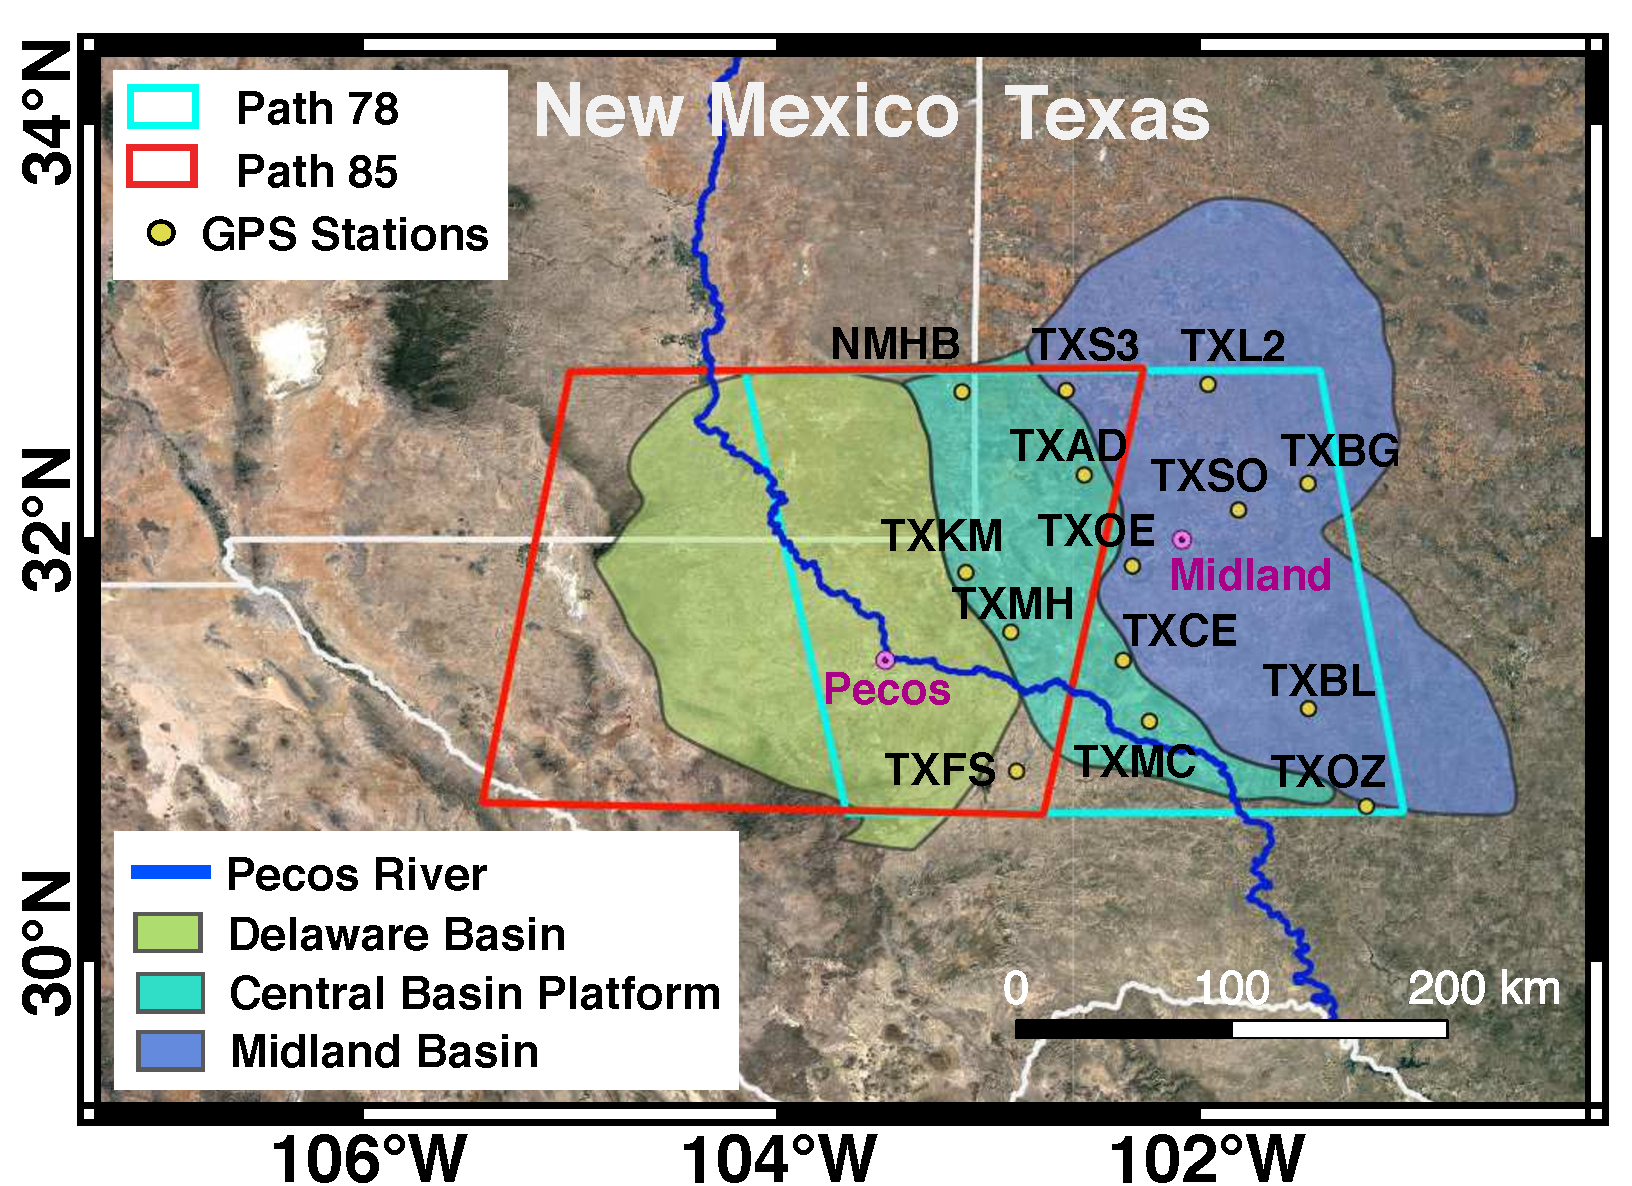
\includegraphics[width=0.9\linewidth]{figure1-study-area.pdf}
\caption{GPS and InSAR data coverage over the Permian Basin. Yellow dots indicate GPS permanent stations. Teal and red boxes indicate ascending path 78 and descending path 85 paths of Sentinel 1 InSAR coverage, respectively. Each path contains over 80 SAR acquisitions, leading to over 3500 interferograms per path at 120 m pixel spacing.}
\label{fig:study-area}
\end{figure}


\begin{figure}[hbt!]
\centering
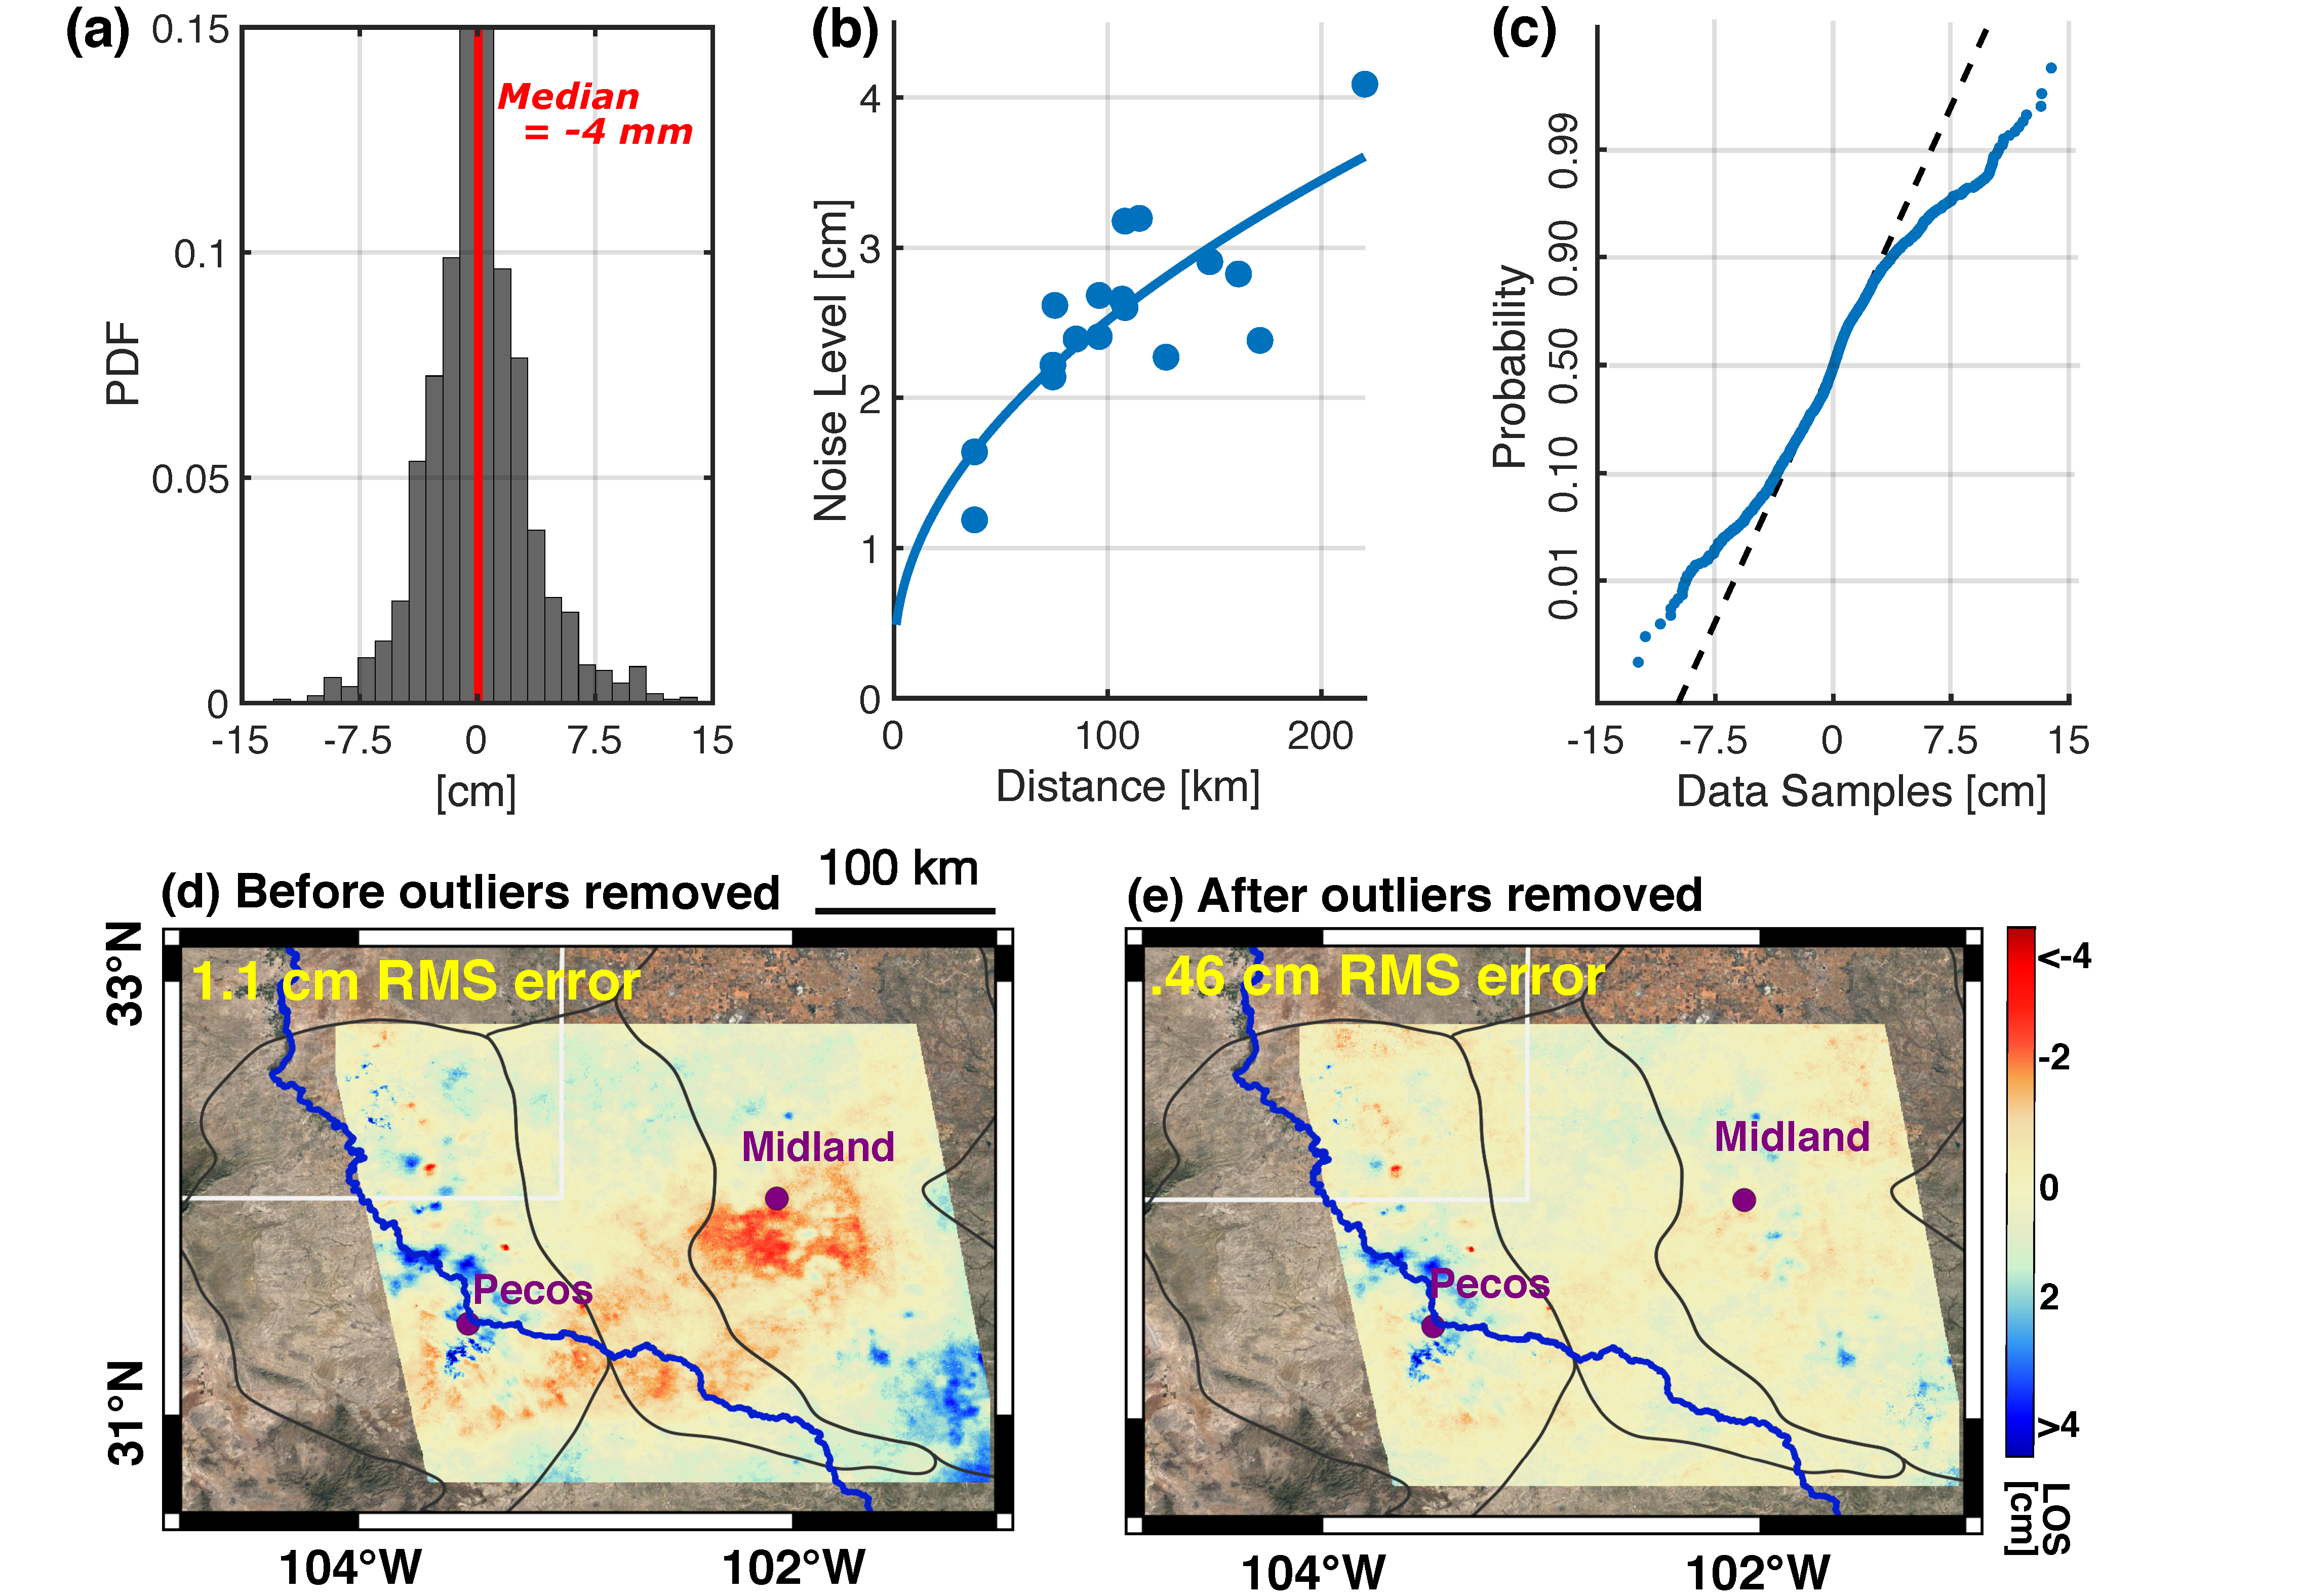
\includegraphics[width=0.95\linewidth]{figure2-outlier-removal-5panel.pdf}
\caption{(a) LOS measurements (in cm) of all ascending interferograms at the GPS station TXMC. The distribution has a near zero median (-4 mm) and a standard deviation of 3.2 cm. Due to the absence of substantial deformation signals, the standard deviation of the distribution is a measure of LOS turbulent tropospheric noise. (b) The standard deviation of random tropospheric turbulent noise at 13 control locations (blue dots), which increases as the square root of the distance from the InSAR reference point (blue line). (c) A comparison between the tropospheric noise distribution at TXMC with a normal distribution. Dashed line connects the 1st and 3rd quartiles of the data. Troposphere noise following a normal distribution would match the dashed line, and non-Gaussian tails (we noted as outliers) are present. Cumulative ascending LOS deformation solutions (Nov. 2014 - Dec. 2017) (d) before and (e) after excluding InSAR outlier measurements. Note that 1.1 cm cumulative error over 3 years is equivalent to 3.5 mm/year RMS error in the velocity estimate.}
\label{fig:outliers}
\end{figure}

\begin{figure*}[hbt!]
\centering
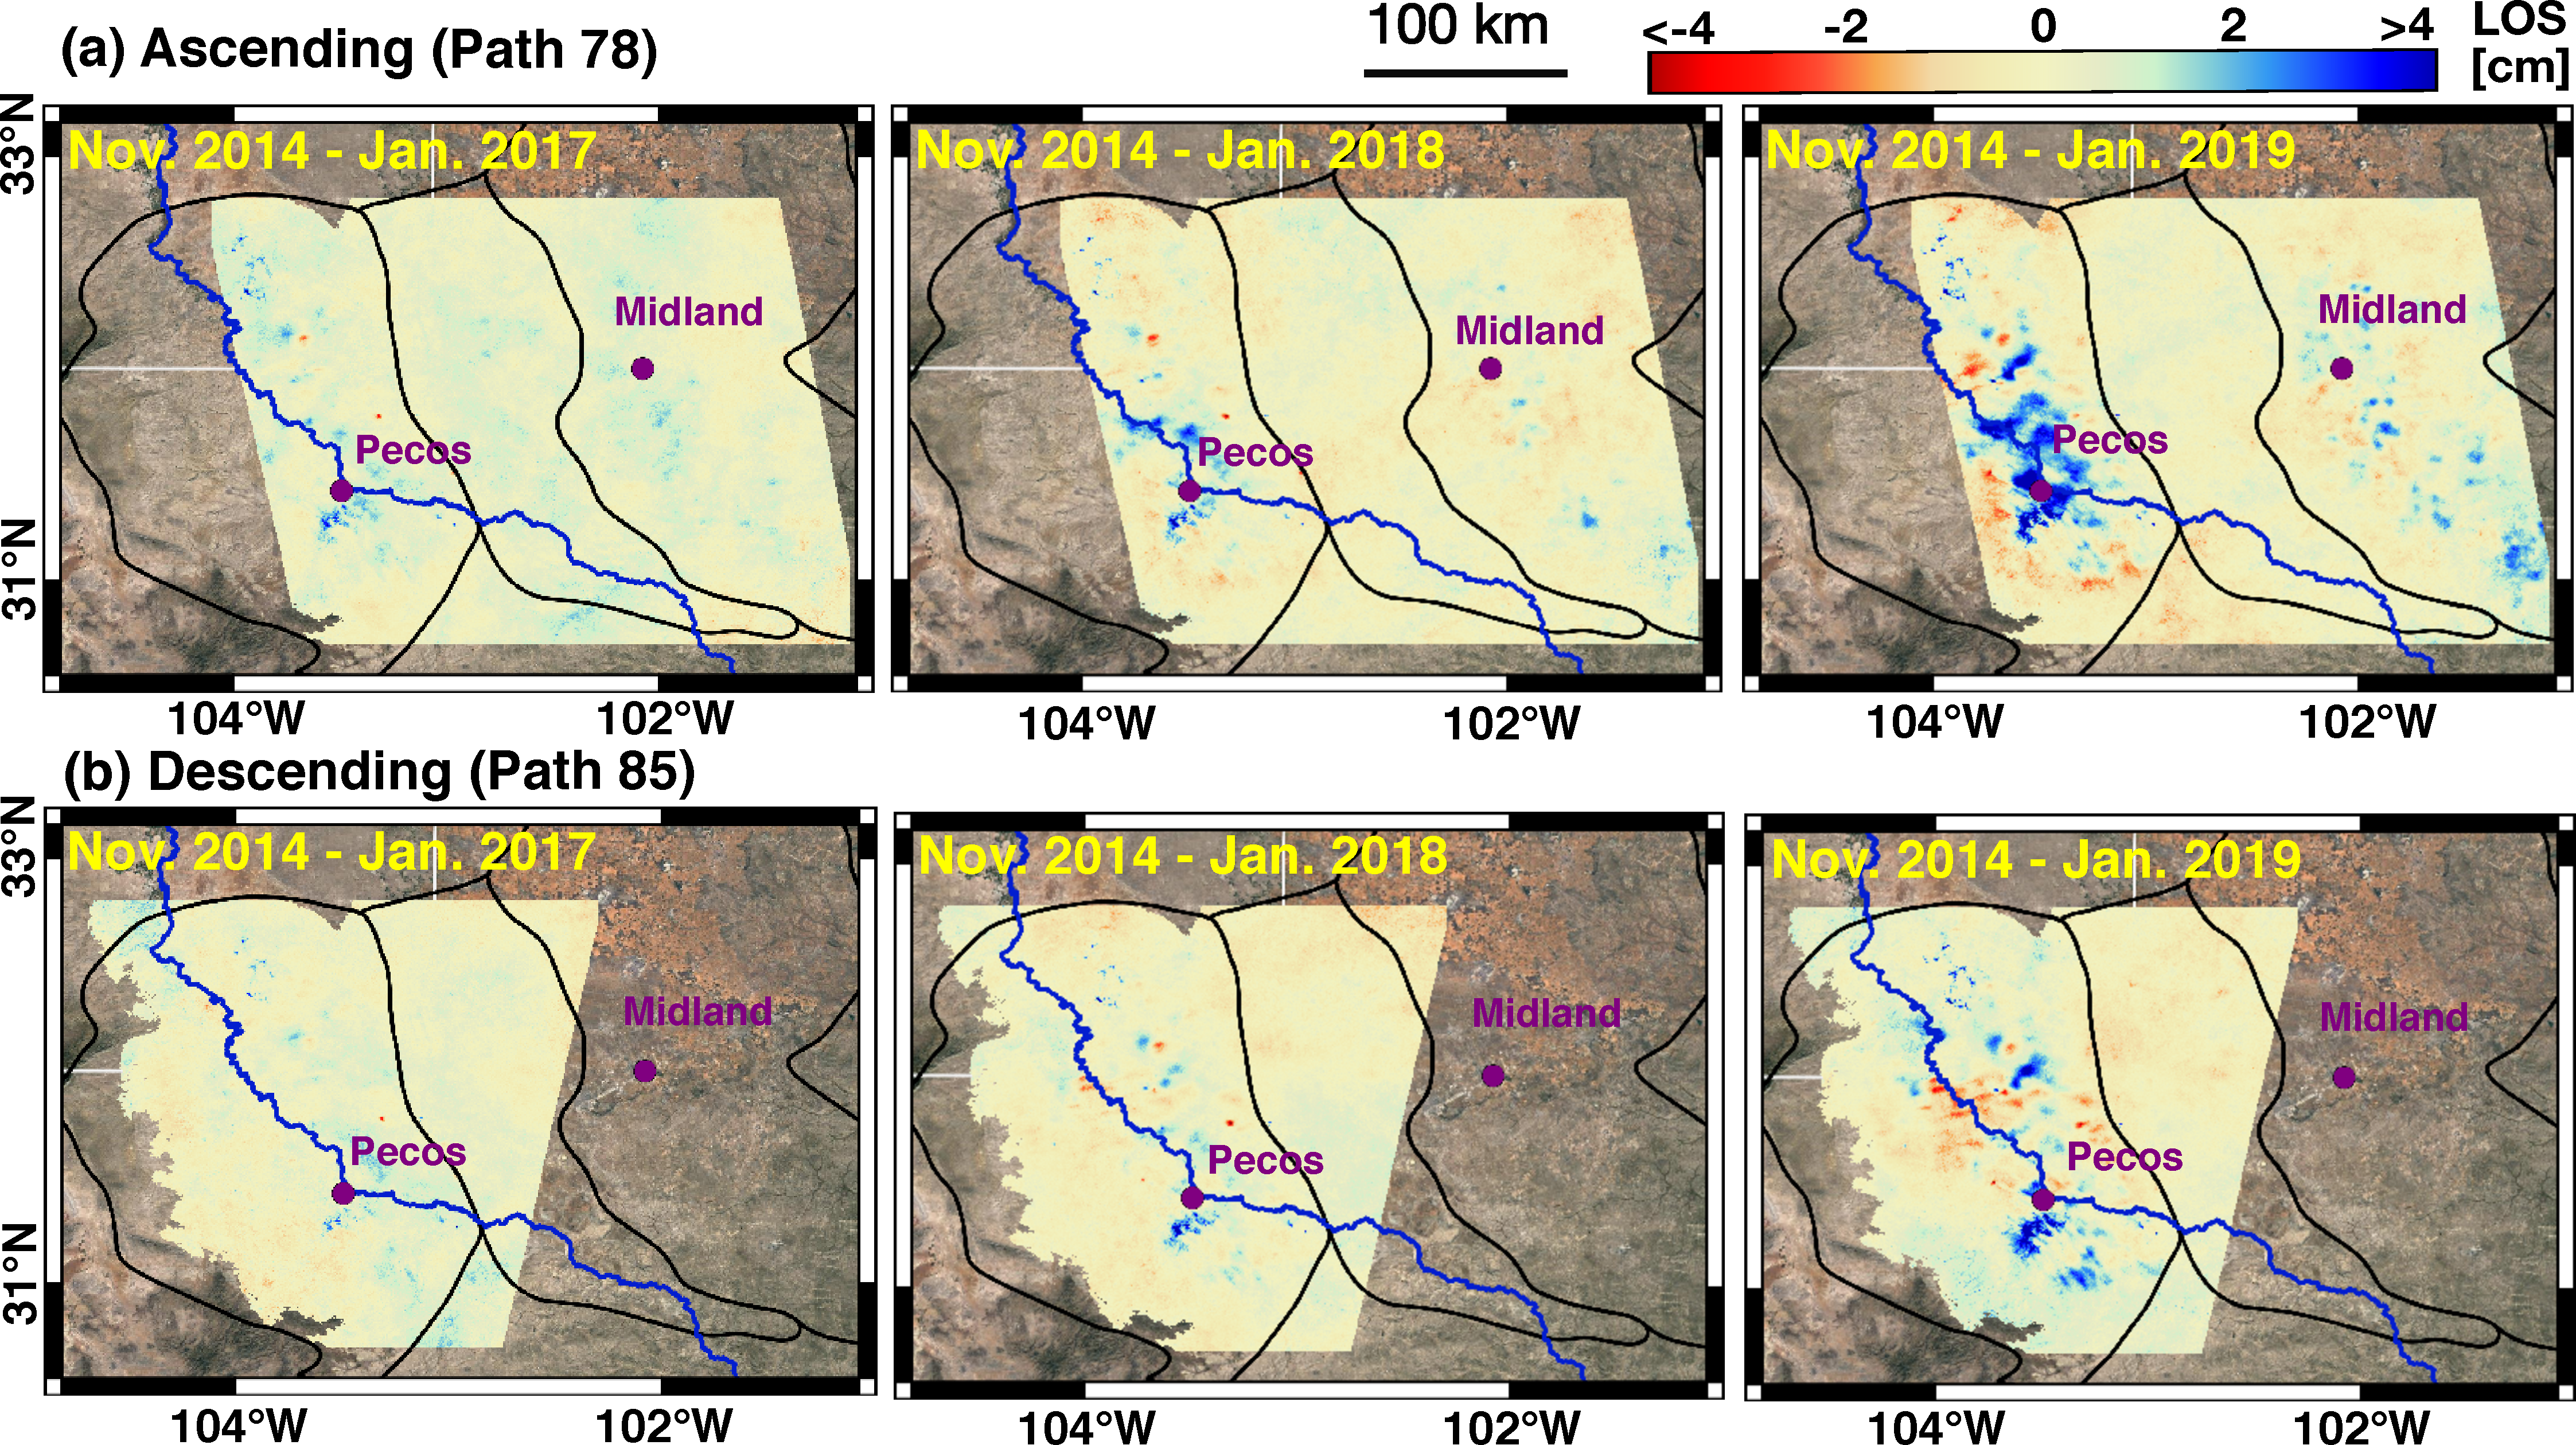
\includegraphics[width=.96\linewidth]{figure3-los-insar.pdf}
\caption{Cumulative LOS deformation (Nov. 2014 - Jan.2017; Nov. 2014 - Jan.2018; Nov. 2014 - Jan. 2019) as inferred from Sentinel-1 (a) ascending path 78, and (b) descending path 85 data over an 80,000 square km oil-producing region of the Permian Basin. Here a subsidence or eastward deformation signal leads to a positive LOS measurement in the ascending geometry, and a subsidence or westward deformation signal leads to a positive LOS measurement in the descending geometry. Areas with $>$1200 m altitude are masked due to the low oil production activity in mountainous regions.}
\label{fig:insar-los}
\end{figure*}

\begin{figure}[hbt!]
\centering
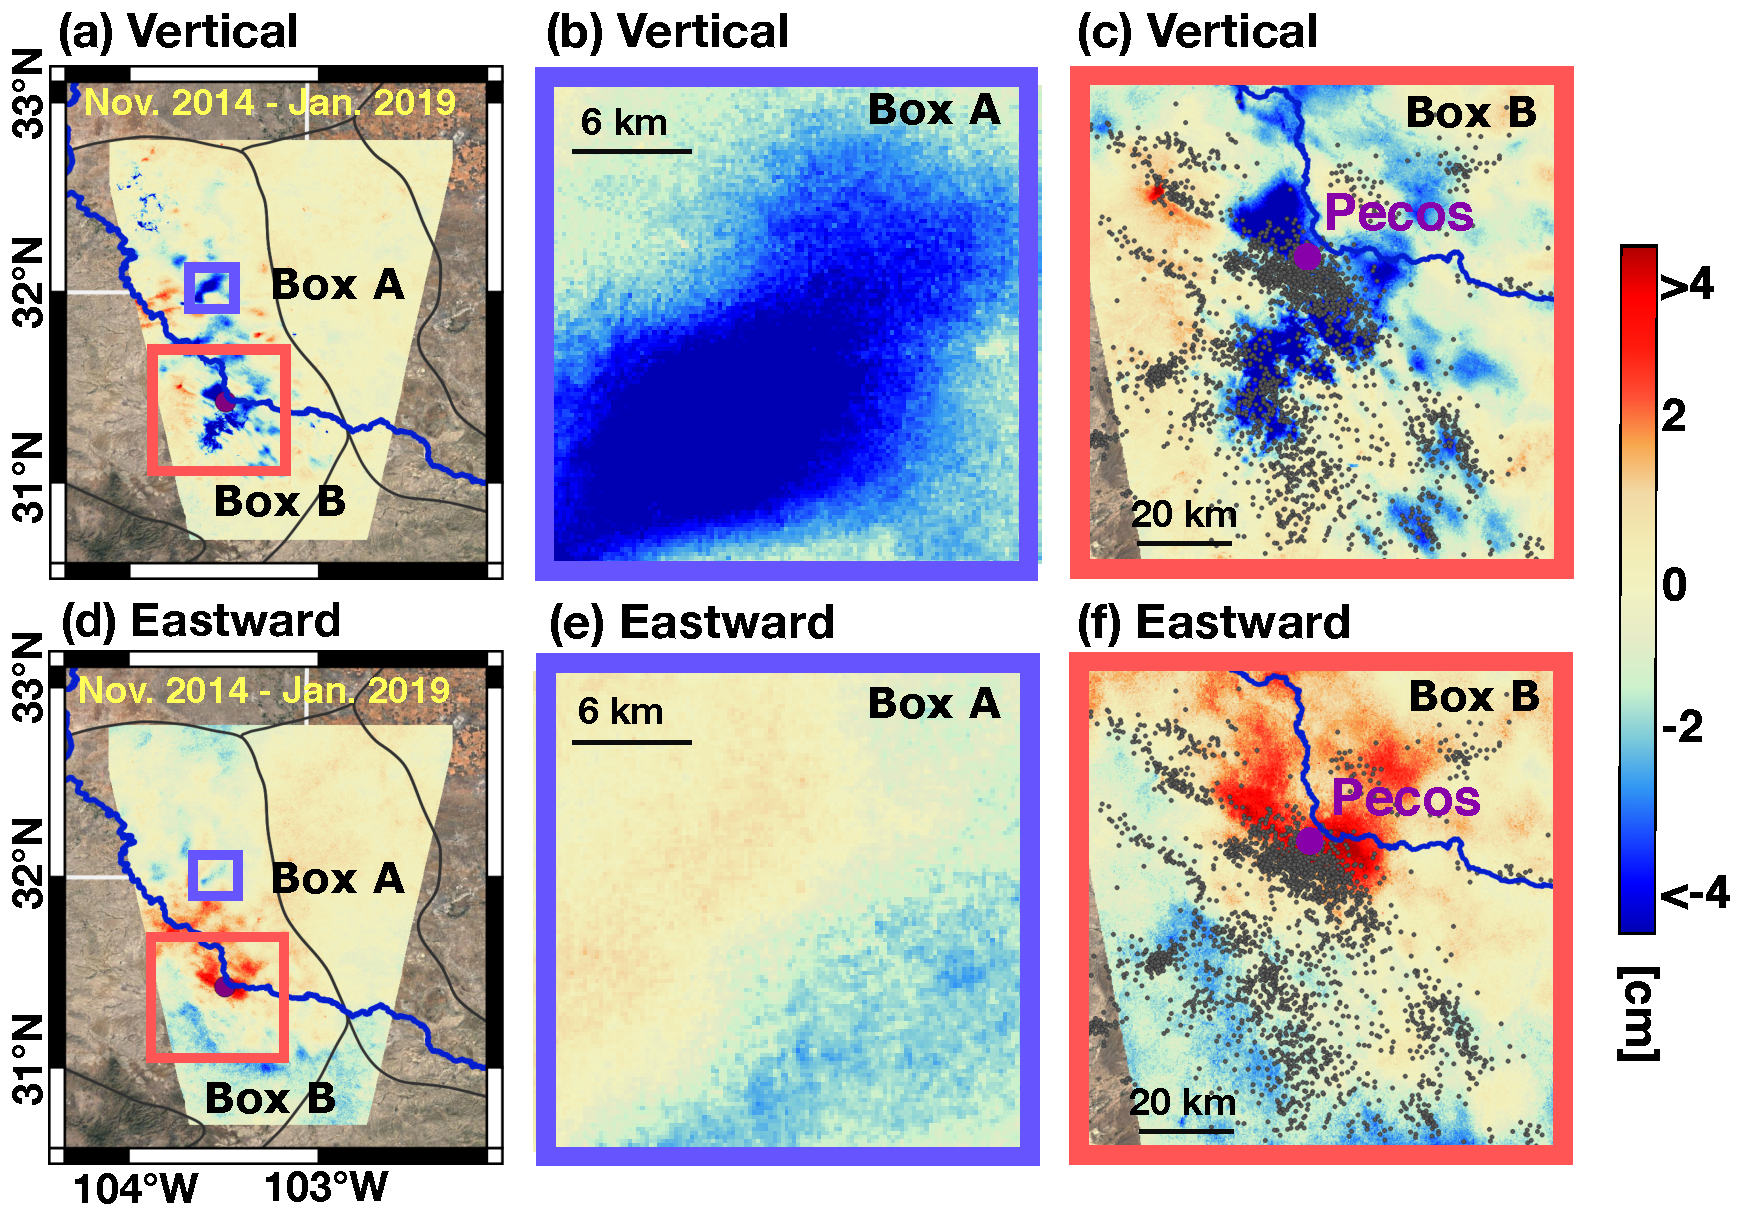
\includegraphics[width=0.96\linewidth]{figure4-east-vertical-6panel-labelled.pdf}
\caption{(a) Cumulative vertical deformation between Nov. 2014 and Jan. 2019 over the region where Sentinel-1 path 78 and path 85 overlap. A zoomed-in view of Box A in the northern Delaware Basin and Box B in the southern Delaware Basin are shown in panel (b) and (c) respectively. (d) Cumulative eastward deformation between Nov. 2014 and Jan. 2019 over the region where Sentinel-1 path 78 and path 85 overlap. A zoomed-in view of Box A in the northern Delaware Basin and Box B in the southern Delaware Basin are shown in panel (e) and (f) respectively. In the southern Delaware Basin, the observed vertical and eastward deformation (panel (c) and (f)) show linear patterns along with earthquake hypocenters (gray dots) detected by TexNet in 2018.}
\label{fig:insar-decomp}
\end{figure}

\begin{figure}[hbt!]
\centering
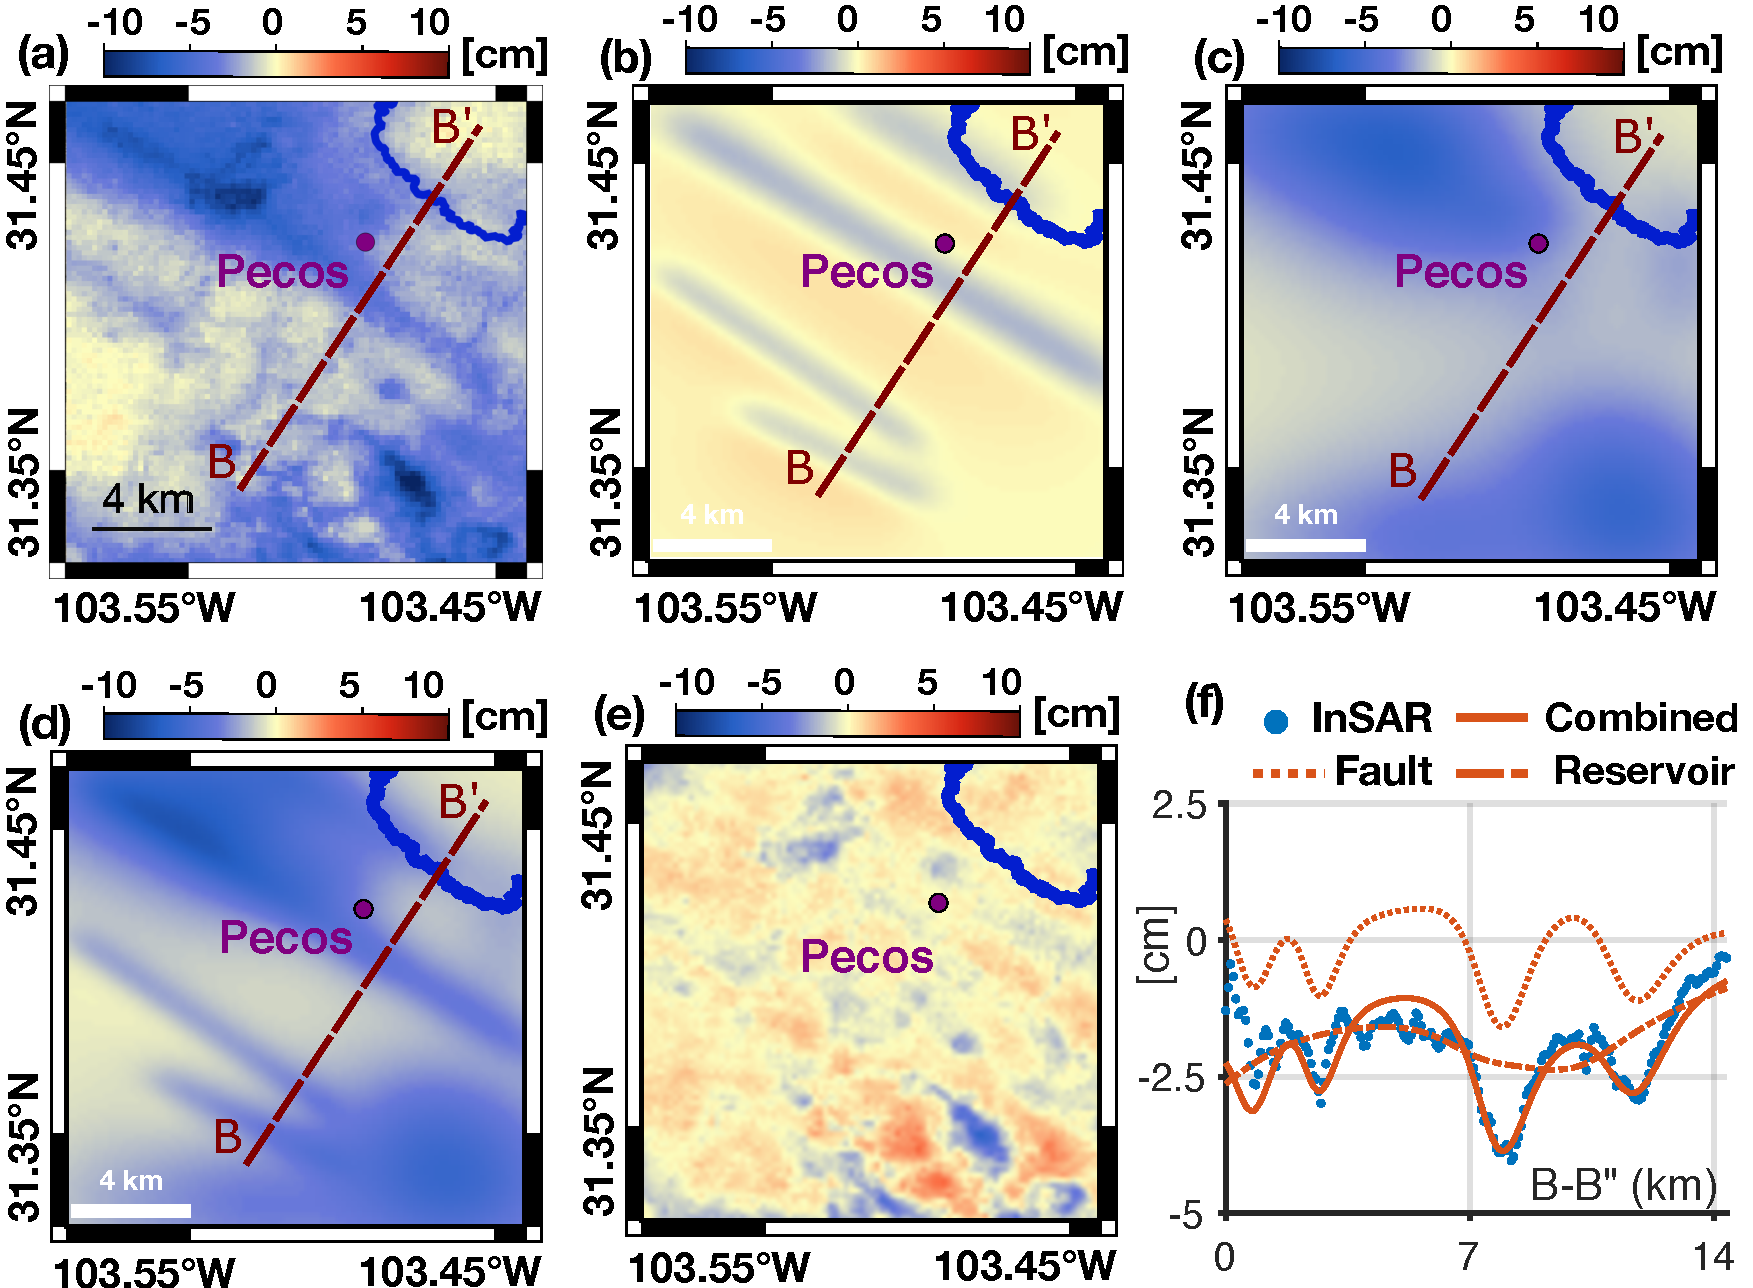
\includegraphics[width=\linewidth]{figure5-modeling.pdf}
\caption{(a) InSAR-observed cumulative vertical deformation between Nov. 2014 and Jan. 2019 in the Pecos, TX area. (b) Modeled vertical deformation associated with four dip-slip faults. (c) Modeled vertical deformation associated with reservoir compaction. (d) Modeled total vertical deformation associated with four dip-slip faults and reservoir compaction (panel (b) $+$ panel (c)). (e) Difference between InSAR-observed and model-predicted vertical deformation (panel (a) $-$ panel (d)). (f) Difference between InSAR-observed and model-predicted vertical deformation along the B-B' transect.}
\label{fig:model}
\end{figure}

\end{document}


